% \documentclass[aspectratio=169,notes]{beamer}
\documentclass[aspectratio=169,xcolor=table]{beamer}
\usetheme[faculty=phil]{fibeamer}
\usepackage{polyglossia}
\setmainlanguage{english} %% main locale instead of `english`, you
%% can typeset the presentation in either Czech or Slovak,
%% respectively.
\setotherlanguages{russian} %% The additional keys allow
%%
%%   \begin{otherlanguage}{czech}   ... \end{otherlanguage}
%%   \begin{otherlanguage}{slovak}  ... \end{otherlanguage}
%%
%% These macros specify information about the presentation
\title[]{Разработка метода тактильного очувствления для мобильного шагающего робота} %% that will be typeset on the
\subtitle{Аспирант: Олег Буличев \\ Руководитель: Александр Малолетов \\ \ } %% title page.
\author{Олег Буличев}
%% These additional packages are used within the document:
\usepackage{ragged2e}  % `\justifying` text
\usepackage{booktabs}  % Tables
\usepackage{tabularx}
\usepackage{tikz}      % Diagrams
\usetikzlibrary{calc, shapes, backgrounds}
\usepackage{amsmath, amssymb}
\usepackage{url}       % `\url`s
\usepackage{listings}  % Code listings
\usepackage{floatrow}
\usepackage{mathtools}
\usepackage{todonotes}
\usepackage{fontspec}
\usepackage{multicol}
\usepackage{pdfpages}
\usepackage{wrapfig}
\usepackage{animate}
\usepackage{booktabs}
\usepackage{multirow}
\usepackage{multimedia}
\usepackage{makecell}
\usepackage{colortbl}
\usepackage{hhline}

\usepackage[font={large}, labelfont=it,textfont={it},justification=centering, skip=2pt]{caption}
% will apply to all subcaptions
\usepackage[font={large},skip=2pt]{subcaption}

\graphicspath{{../images/}}
\frenchspacing


\usetikzlibrary{decorations.pathreplacing,calligraphy,calc,graphs}

\setbeamertemplate{caption}[numbered]

% \usepackage[backend=biber,style=ieee,autocite=footnote]{biblatex}
% \addbibresource{biblio.bib}
% \DefineBibliographyStrings{english}{%
%   bibliography = {References},}

\newcommand{\oleg}[2][] {\todo[color=red, #1] {OLEG:\\ #2}}
\newcommand{\fbckg}[1]{\usebackgroundtemplate{\includegraphics[width=\paperwidth]{#1}}}%frame background

\usepackage[framemethod=TikZ]{mdframed}
\newcommand{\dbox}[1]{
\begin{mdframed}[roundcorner=3pt, backgroundcolor=yellow, linewidth=0]
\vspace{1mm}
{#1}
\vspace{1mm}
\end{mdframed}
}

\begin{document}
\setlength{\abovedisplayskip}{0pt}
\setlength{\belowdisplayskip}{0pt}
\setlength{\abovedisplayshortskip}{0pt}
\setlength{\belowdisplayshortskip}{0pt}

\fbckg{fibeamer/figs/title_page.png}
\frame[c]{\setcounter{framenumber}{0}
    \usebeamerfont{title}%
    \usebeamercolor[fg]{title}%
    \begin{minipage}[b][7.5\baselineskip][b]{\textwidth}%
        \textcolor{black}{\raggedright\inserttitle}
    \end{minipage}
    % \vskip-1.5\baselineskip

    \usebeamerfont{subtitle}%
    \usebeamercolor[fg]{framesubtitle}%
    \begin{minipage}[b][3\baselineskip][b]{\textwidth}
        \raggedright%
        \insertsubtitle%
    \end{minipage}
    \vskip.25\baselineskip
}
%   \frame[c]{\maketitle}

\fbckg{fibeamer/figs/common.png}

\begin{frame}[t]{О себе}
\framesubtitle{}
    \begin{exampleblock}{Образование}
        \begin{itemize}
            \item Бакалавриат --- МГТУ им. Н.Э. Баумана, РК6 (красный диплом) \\ \textbf{Тема:} Разработка системы управления наведением МРК <<Пластун>>
            \item Магистратура --- Университет Иннополис, Робототехника \\ \textbf{Тема:} Development of biomimetic centipede robot <<StriRus>>
            \item Аспирантура --- Университет Иннополис, Робототехника
        \end{itemize}
    \end{exampleblock}
    \begin{alertblock}{Текущие должности}
        \begin{itemize}
        \item Старший преподаватель (Лин. Алг., Теор. Мех., МиМ)
        \item Инженер-исследователь
    \end{itemize}
    \end{alertblock}
\end{frame}

\begin{frame}[t]{Цель работы}
\framesubtitle{}
\vspace{-0.4cm}
    Определить \underline{геометрические} и \underline{физические} свойства пройденной \textbf{поверхности} с помощью шагающего движителя, используя \textit{тактильное очувствление}.

\begin{figure}[H]
    \begin{subfigure}{0.49\textwidth}
        \centering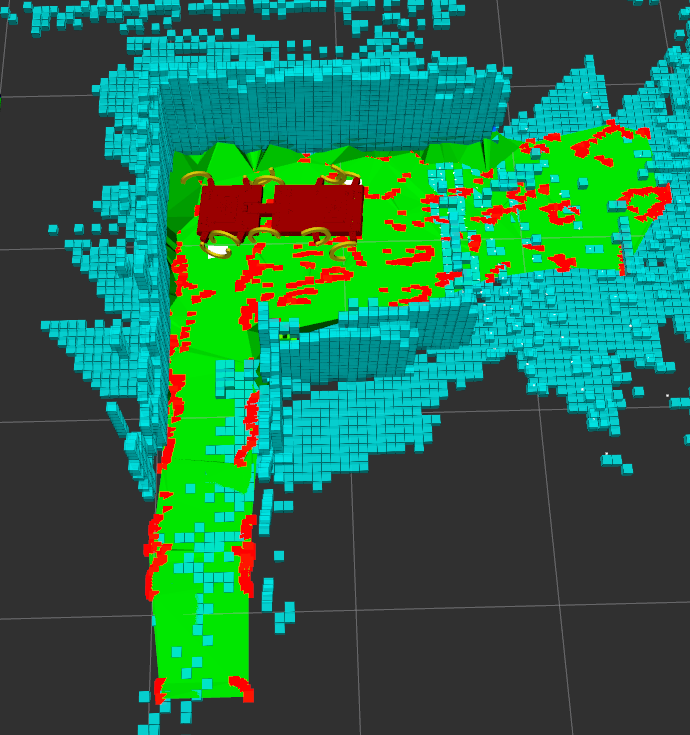
\includegraphics[height=4.5cm,width=1\textwidth,keepaspectratio]{conv_concave.png}
        \caption*{Определение геометрических свойств}
    \end{subfigure}
    \begin{subfigure}{0.49\textwidth}
        \centering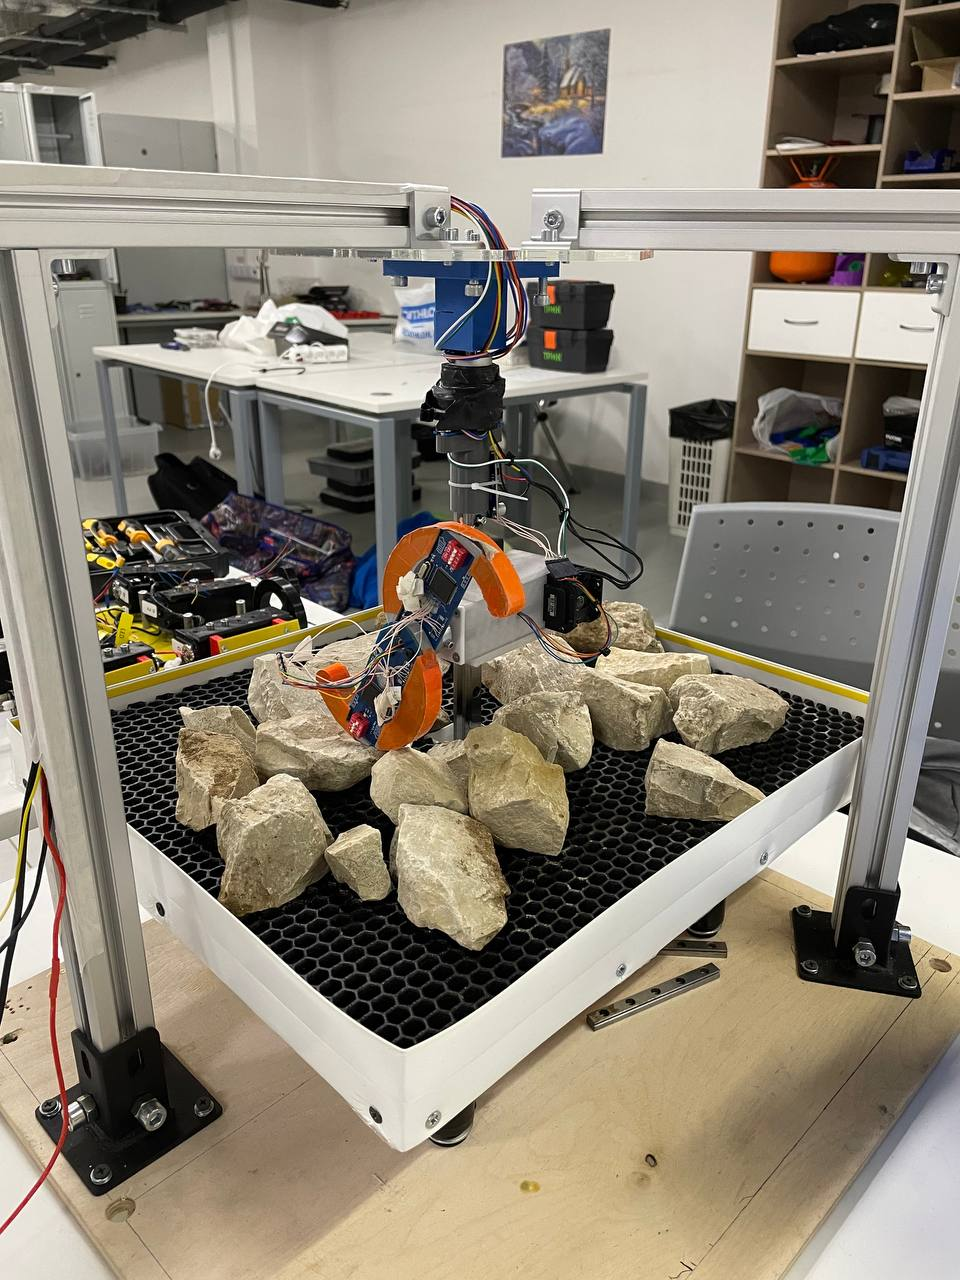
\includegraphics[height=4.5cm,width=1\textwidth,keepaspectratio]{s_shape_leg/view.jpg}
        \caption*{Определение физических свойств}
        \label{fig:s_shape_leg/view.jpg}
    \end{subfigure}
\end{figure}

\end{frame}

\begin{frame}[t]{Нерешаемая задача с помощью камеры или лидара}
    \framesubtitle{Вопрос: Как картографировать поверхность под лужей?}
    \vspace{-1cm}
    \begin{columns}[T,onlytextwidth]
        \begin{column}{0.55\textwidth}


            \begin{figure}[H]
                \centering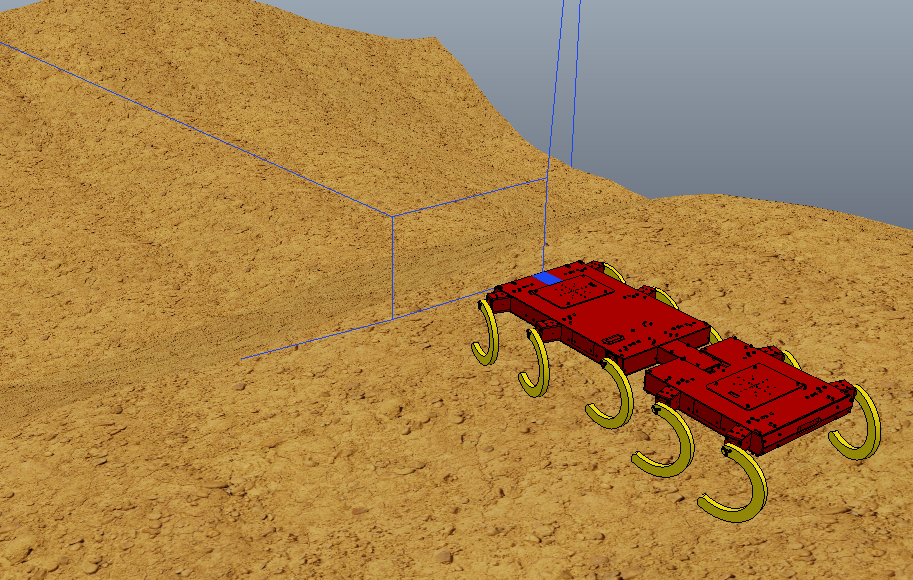
\includegraphics[height=6cm,width=1\textwidth,keepaspectratio]{terrain_wo_water.png}
                \caption*{Поверхность без воды}
            \end{figure}
        \end{column}
        \begin{column}{0.44\textwidth}
            \begin{figure}[H]
                \begin{subfigure}[b]{0.9\textwidth}
                    \centering
                    \begin{tikzpicture}
                        % Include the image in a node
                        \node [above right, inner sep=0] (image) at (0,0)
                        {\centering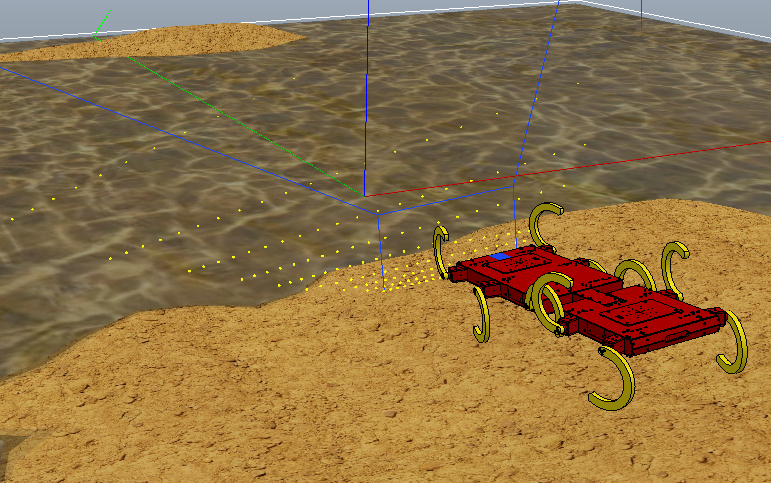
\includegraphics[height=3.5cm,width=1\textwidth,keepaspectratio]{terrain_w_water1.png}};
                        % Create scope with normalized axes
                        \begin{scope}[
                                x={($ 0.1*(image.south east)$)},
                                y={($ 0.1*(image.north west)$)}]
                            % Grid and axes' labels
                            % \draw[lightgray,step=1] (image.south west) grid (image.north east);
                            % \foreach \x in {0,1,...,10} { \node [below] at (\x,0) {\x}; }
                            % \foreach \y in {0,1,...,10} { \node [left] at (0,\y) {\y};}
                            % Labels
                            \draw[stealth-, very thick,green] (6,8) -- ++(2,1)
                            node[rounded corners=3pt,right,black,fill=white]{\tiny Water};

                            \draw[stealth-, very thick,green] (0.5,5.5) -- (3,2);
                            \draw[stealth-, very thick,green] (2.5,4.2) -- (3,2);
                            \draw[stealth-, very thick,green] (4.5,4) -- (3,2)
                            node[rounded corners=3pt,below,black,fill=white]{\tiny Lidar data};
                        \end{scope}
                    \end{tikzpicture}
                    % \caption*{}
                    \label{fig:terrain_w_water1.png}
                \end{subfigure}
                \vspace{-0.5cm}

                \begin{subfigure}{0.8\textwidth}
                    \centering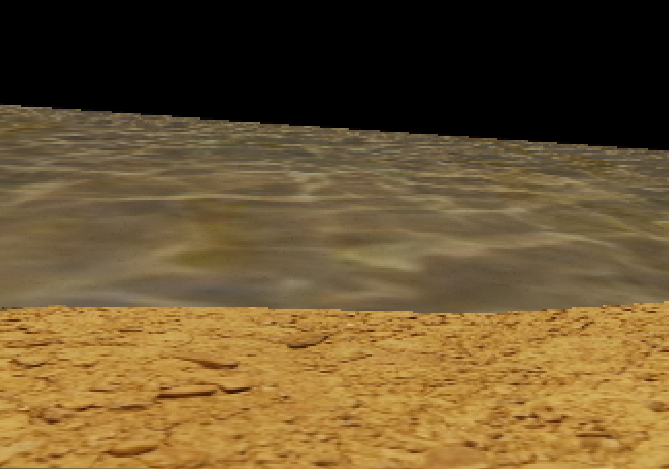
\includegraphics[height=2cm,width=1\textwidth,keepaspectratio]{terrain_w_water_camera.png}
                    \caption*{Вид с камеры}
                \end{subfigure}
            \end{figure}
        \end{column}
    \end{columns}

\end{frame}

\begin{frame}[t]{Актуальность проблематики}
\framesubtitle{}
\begin{figure}[H]
    \begin{subfigure}[t]{0.32\textwidth}
        \centering
\includegraphics[height=4cm,width=1\textwidth,keepaspectratio]{Darpa_SubT.png}
        \caption*{Соревнование по автономному исследованию пещер}
        \label{fig:Darpa_SubT.png}
    \end{subfigure}
    \begin{subfigure}[t]{0.32\textwidth}
        \centering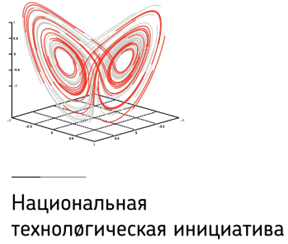
\includegraphics[height=4cm,width=1\textwidth,keepaspectratio]{NTI.png}
        \caption*{Спонсирование проекта по тематике}
        \label{fig:NTI.png}
    \end{subfigure}
    \begin{subfigure}[t]{0.32\textwidth}
        \centering
\includegraphics[height=4cm,width=1\textwidth,keepaspectratio]{rffi.jpeg}
        \caption*{Грант по тематике}
        \label{fig:rffi.jpeg}
    \end{subfigure}
\end{figure}
\end{frame}


\begin{frame}[t]{Литературный обзор}
    \framesubtitle{}
    \vspace{-0.65cm}
    \begin{itemize}
        \item Пещеры: препятствия, размеры. \\ \alert{-- \textbf{Классификация} пещер и препятствий \\ -- \textbf{Оценка сложности} территории}
        \item Роботы для исследования пещер: от дирижаблей, до шагающих. \\ \alert{-- \textbf{Робототехнические системы} для исследования \textbf{свободных пещер}}
        \item Способы определения силы реакции опоры. \\ \alert{-- Неявные и явные \textbf{способы}. \textbf{Классификая типов датчиков} силы}
        \item Методы распознования типа поверхности. \\ \alert{-- С помощью \textbf{машинного обучения}, используя набор датчиков}
        \item Методы построения карты: оптические и тактильные. \\ \alert{-- Построение поверхности \textbf{с помощью датчика силы на манипуляторе} \\ -- Построение карты с помощью \textbf{лидаров и камер}}
    \end{itemize}

\end{frame}

\begin{frame}[t]{Разработка робота}
    \framesubtitle{Требования к роботу}
    \large
\vspace{-0.5cm}
    \begin{columns}[T,onlytextwidth]
        \begin{column}{0.49\textwidth}
            \textbf{Задача} --  выбрать движитель. Робот должен:
            \begin{itemize}
                \item Иметь \textit{малые размеры}, чтобы лазать и не застевать в щелях
                \item Обладать \textit{проходимостью} для преодоления сыпучих грунтов
                \item Преодолевать \textit{небольшие водные препятствия}
                \item Иметь возможнсоть \textit{залезать на большие валуны}
            \end{itemize}        
        \end{column}
        \begin{column}{0.49\textwidth}
            \vspace{-1.1cm}
            \begin{figure}[H]
                \centering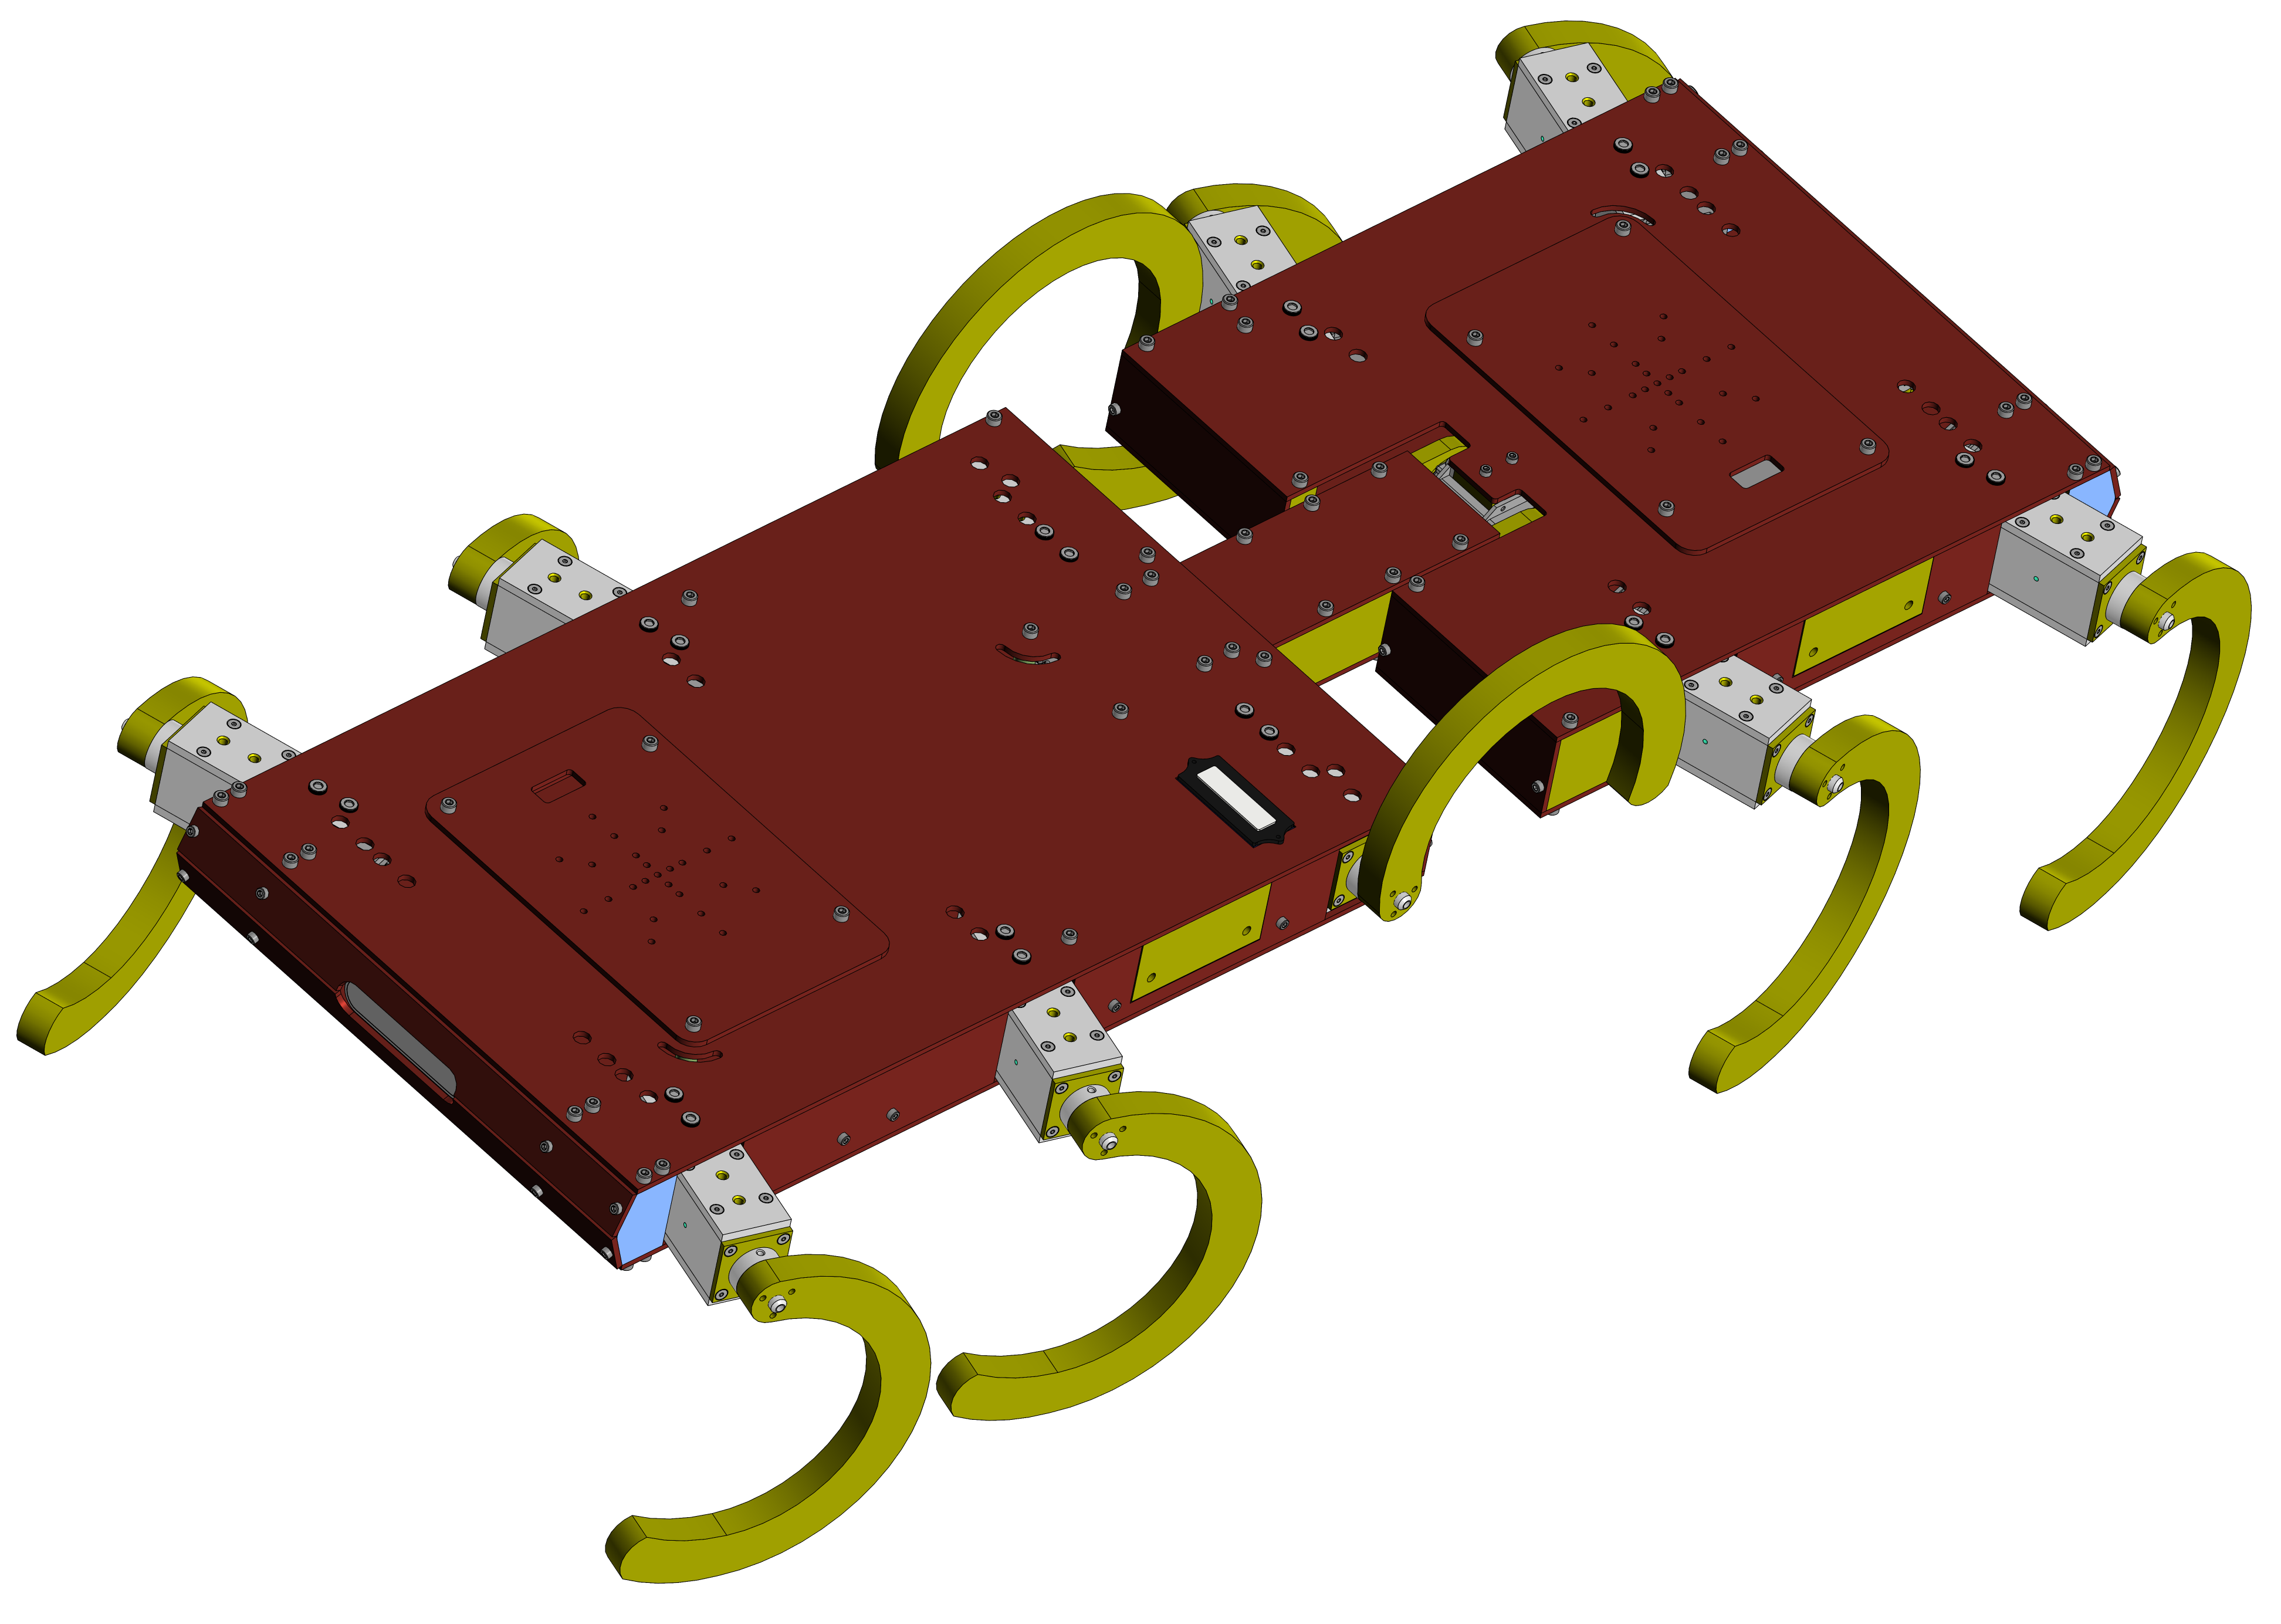
\includegraphics[height=5cm,width=1\textwidth,keepaspectratio]{strirus_4.png}
                \caption*{Шагающий цикловой движитель с 1 степенью свободы в ноге \\ \textbf{СтриРус}, 4-ая итерация}
                \label{fig:strirus_4.png}
            \end{figure}
        \end{column}
    \end{columns}
\end{frame}

\begin{frame}[t]{Разработка робота}
    \framesubtitle{Видео}
    \vspace{-0.6cm}
    \begin{figure}[H]
        % \href{run:./videos/sidestep_segments.mp4}{
        \href{https://youtu.be/EQ6oGZVDpoc}{
            \centering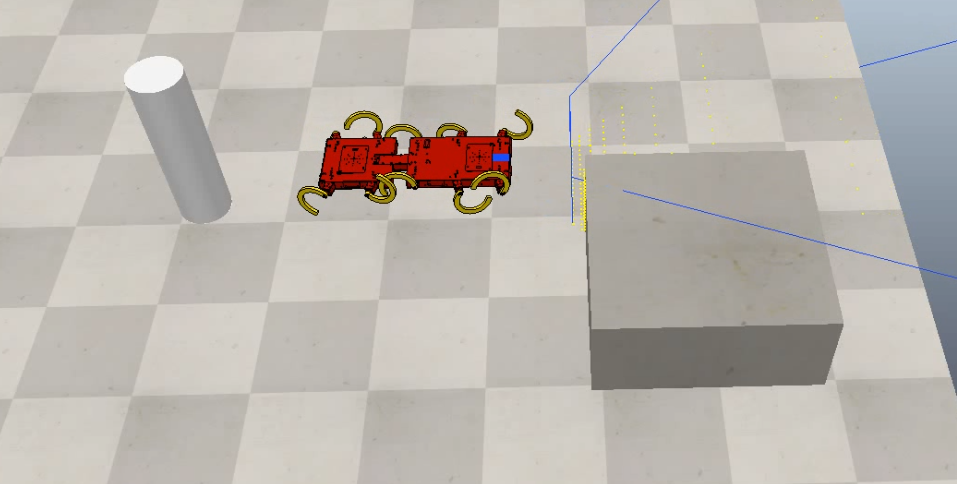
\includegraphics[height=6cm,width=1\textwidth,keepaspectratio]{sidestep_segment_video_preview.png}}
        % \caption{Click on a picture for a video}
    \end{figure}
\end{frame}

\begin{frame}[t]{Разработка робота}
    \framesubtitle{Структурный синтез}
    {\large\begin{block}{Вопрос}
            Какое оптимальное количество ног должен иметь такой движитель?
        \end{block}}
    {\large\begin{alertblock}{Ответ}
            \centering Решив задачу структурного синтеза,\\ результатом которого является движитель с \textbf{8---14 ногами}
        \end{alertblock}}
\end{frame}

\begin{frame}[c]{Разработка робота}
    \framesubtitle{Используемые технологии}
    \vspace{-0.7cm}
    \begin{figure}[H]
        \begin{subfigure}[t]{0.32\textwidth}
            \centering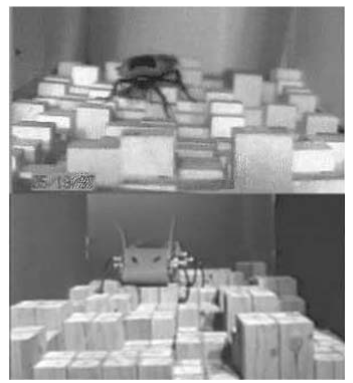
\includegraphics[height=4cm,width=1\textwidth,keepaspectratio]{c1_paper.png}
            \caption*{\small Генерация поверхности \\ (Параметризованная \textbf{искусственная территория}) \\ \alert{Проблема формализации сложности поверхности}}
        \end{subfigure}
        \hfill
        \begin{subfigure}[t]{0.32\textwidth}
            \centering
\includegraphics[height=4cm,width=1\textwidth,keepaspectratio]{gazebo_logo.png}
            \caption*{\small Робосимулятор \\ (Неявная математическая модель) \\ \alert{Громоздкость явной модели}}
        \end{subfigure}
        \hfill
        \begin{subfigure}[t]{0.32\textwidth}
            \centering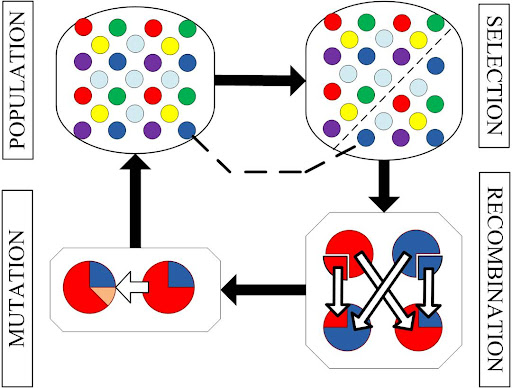
\includegraphics[height=5.5cm,width=1\textwidth,keepaspectratio]{gen_algo.jpg}
            \caption*{ \small Генетический алгоритм \\ \alert{Отличен для \\ дискретной глобальной \\ мультикретиральной задачи оптимизации}}
        \end{subfigure}
        \hfill
    \end{figure}
\end{frame}

\begin{frame}[t]{Разработка робота}
    \framesubtitle{Предлагаемое решение}
    \begin{columns}[T,onlytextwidth]
        \begin{column}{0.48\textwidth}
            \begin{figure}[H]
                \centering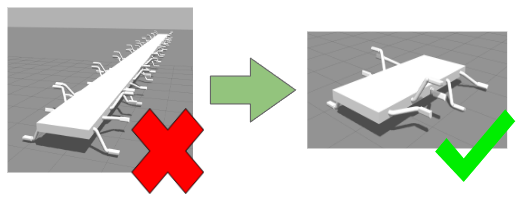
\includegraphics[height=3cm,width=1\textwidth,keepaspectratio]{optimization_idea.png}
                \caption*{\textbf{Идея}: Минимизировать кол-во ног без потери проходимости}
                \label{fig{optimization_idea.png}}
            \end{figure}
        \end{column}
        \begin{column}{0.50\textwidth}
            \vspace{-2cm}
            \begin{figure}[H]
                \centering
                \begin{tikzpicture}
                    % Include the image in a node
                    \node [above right, inner sep=0] (image) at (0,0)
                    {\centering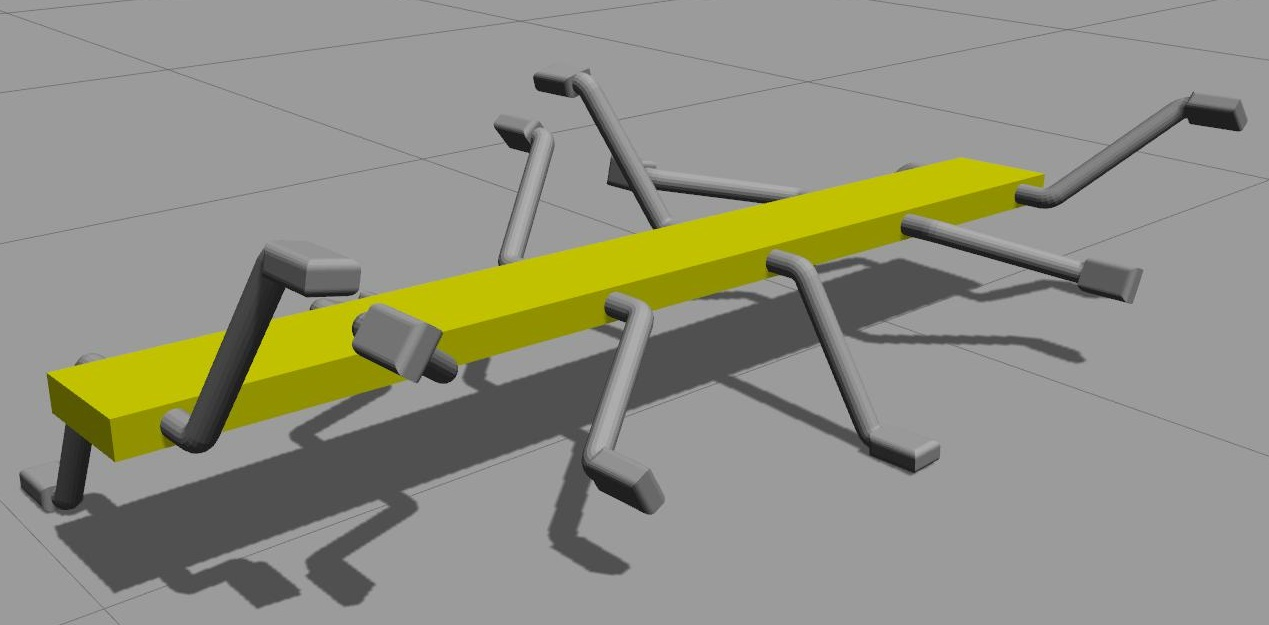
\includegraphics[height=2.5cm,width=1\textwidth,keepaspectratio]{best_gen_robot.jpg}};
                    % Create scope with normalized axes
                    \begin{scope}[
                            x={($ 0.1*(image.south east)$)},
                            y={($ 0.1*(image.north west)$)}]
                        % Grid and axes' labels
                        % \draw[lightgray,step=1] (image.south west) grid (image.north east);
                        % \draw[lightgray,step=0.5] (image.south west) grid (image.north east);
                        % \foreach \x in {0,1,...,10} { \node [below] at (\x,0) {\x}; }
                        % \foreach \y in {0,1,...,10} { \node [left] at (0,\y) {\y};}

                        % Labels
                        \draw [green, very thick,
                            decorate,
                            decoration = {brace,
                                    raise=5pt,
                                    amplitude=5pt,
                                    aspect=0.5}] (1.4,3.6) --  (8.1,6.8)
                        node[rounded corners=3pt, pos=0.5,above left =14pt,black,fill=white]{\tiny $(\gamma - 1) h_{\text{leg}}sin(\alpha)$};

                        \draw[stealth-, very thick,green] (9.5,7.8) -- (7.8,1.94);
                        \draw[stealth-, very thick,green] (1.5,2.8) -- (7,1)
                        node[rounded corners=3pt,right,black,fill=white]{\tiny $\gamma = 6$};

                        \draw[thin,green] (6.7,4) -- (5.75,9);
                        \draw[thin,green] (4.85,3.5) -- (5.75,9);
                        \draw[thin,green,stealth-stealth] (6.32,6) arc (-79.2:-99.2:3) node [rounded corners=3pt,below = 2pt,black,fill=white, midway] {\tiny $\alpha$};
                    \end{scope}
                \end{tikzpicture}
                % \caption*{}
                \label{fig:best_gen_robot.jpg}
            \end{figure}
            \vspace{-1cm}
            {\footnotesize
                \begin{eqnarray*}
                    % \resizebox{0.9\hsize}{!}{
                    F \rightarrow max = \beta \left( {\omega}_{1} \cdot \overbrace{\delta}^{\text{Дистанция}} + {\omega}_{2} \cdot \overbrace{\frac{1}{(\gamma - 1) h_{\text{leg}}sin(\alpha)}}^{\text{Упр. длина корпуса}}\right) +\\ \nonumber + (1 - \beta) {\delta}^{{\omega}_{1}} {\left( \frac{1}{(\gamma - 1)h_{\text{leg}}sin(\alpha)}\right)}^{{\omega}_{2}}
                    % }
                \end{eqnarray*}
            }
            % \vspace{1pt}

            $\beta$ -- адаптивный параметр, \\ ${\omega}_{1,2} \in  [ 0..1 ] $ -- весовые коэффициенты.
        \end{column}
    \end{columns}
\end{frame}

\begin{frame}[t]{Разработка робота}
    \framesubtitle{Видео: История одного сгенерированного робота}
    \vspace{-0.6cm}
    \begin{figure}[H]
        % \href{run:./videos/pass_rand_terr.mp4}{
        \href{https://youtu.be/DcovvkTZgsg}{
            \centering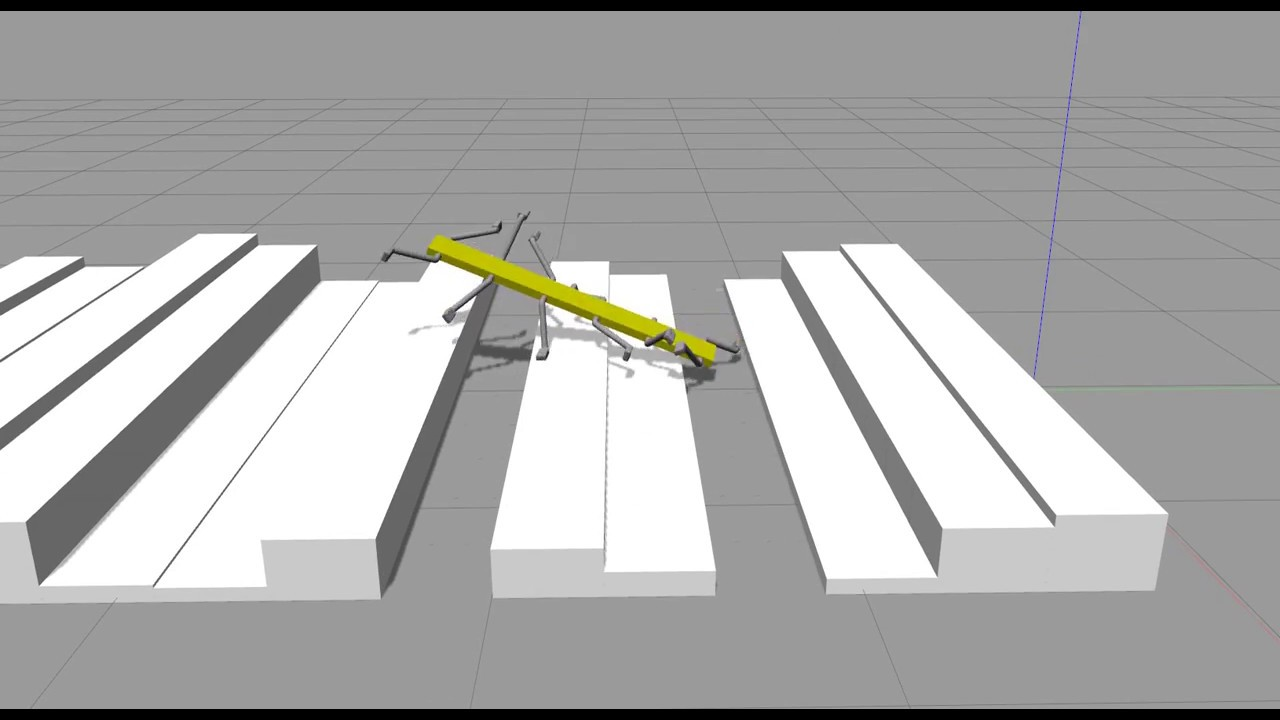
\includegraphics[height=6cm,width=1\textwidth,keepaspectratio]{genetic_video_preview.jpg}}
        % \caption{Click on a picture for a video}
    \end{figure}
\end{frame}

\begin{frame}[t]{Разработка робота}
    \framesubtitle{Конкретные результаты: $\omega_1 = 0.6$, $\omega_2 = 0.4$}
    \vspace{-0.6cm}

    \begin{table}[H]
        \centering
        \begin{tabular}{c|c|c|c|c}
         & \textbf{\begin{tabular}[c]{@{}c@{}}Тип\\ территории\end{tabular}} & \textbf{Кол-во ног} & \textbf{\begin{tabular}[c]{@{}c@{}}Угол между\\ соседними ногами\end{tabular}} & \textbf{Кол-во индивидов} \\
         \hline
         \rule{0cm}{0.5cm}
        \textbf{Этап 1} &  & \cellcolor[HTML]{DAE8FC}12 & 73 & 200 \\ \cline{1-1} \cline{3-5} 
         & \multirow{-2}{*}{\begin{minipage}{2.5cm}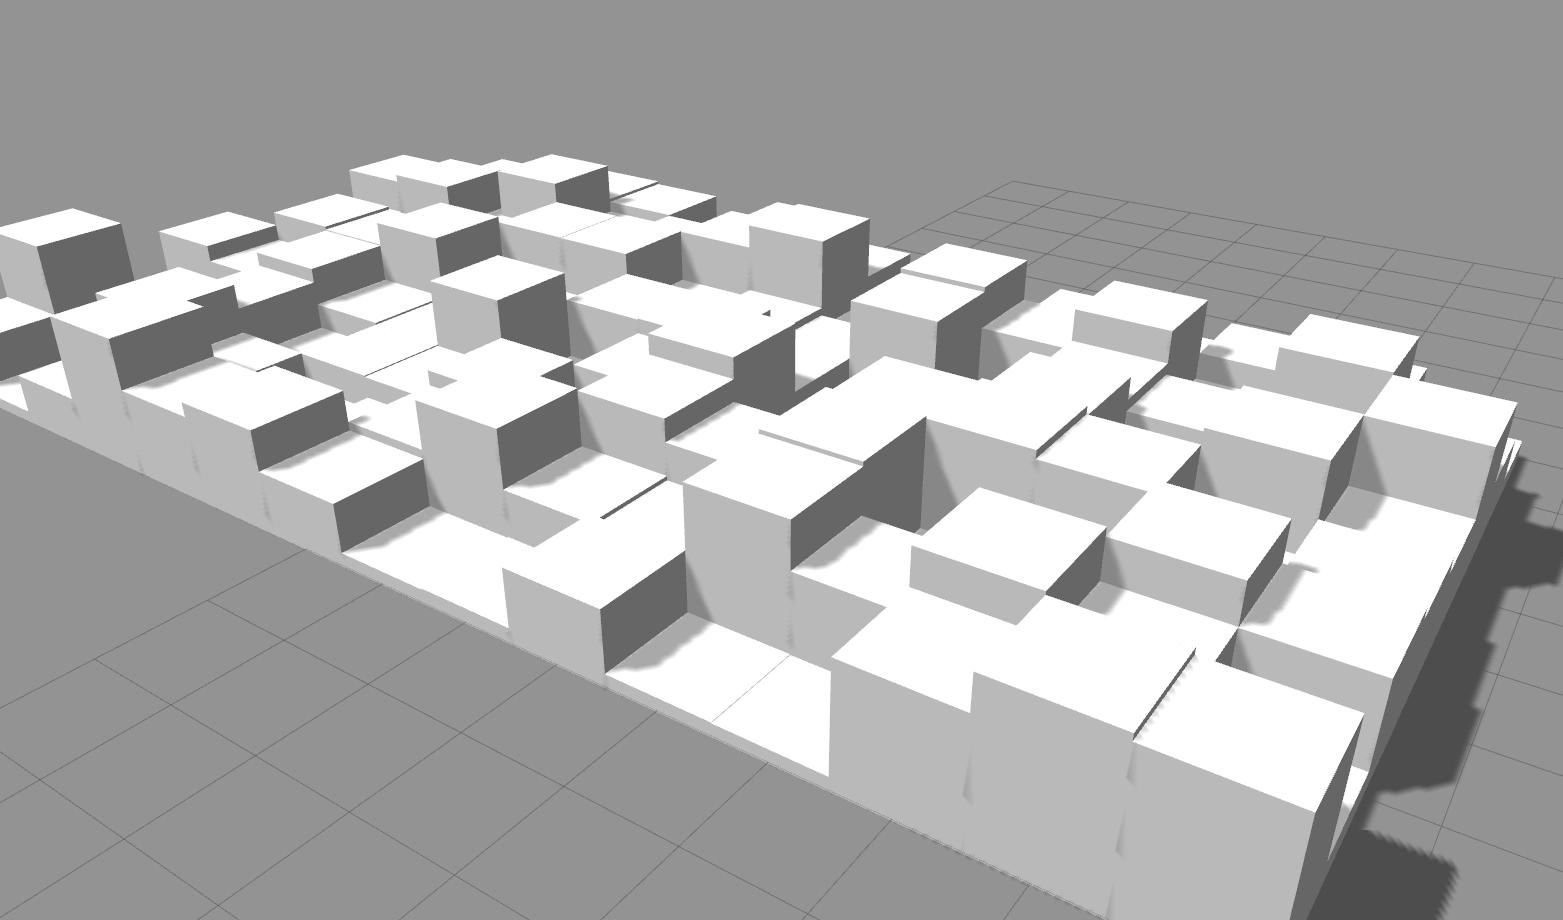
\includegraphics[height=3cm,width=2.5cm,keepaspectratio]{terrain_1.jpg}\end{minipage}} & \cellcolor[HTML]{DAE8FC}12 & 72 &  \\ [0.5cm] \cline{3-4} 
         & \begin{minipage}{2.5cm}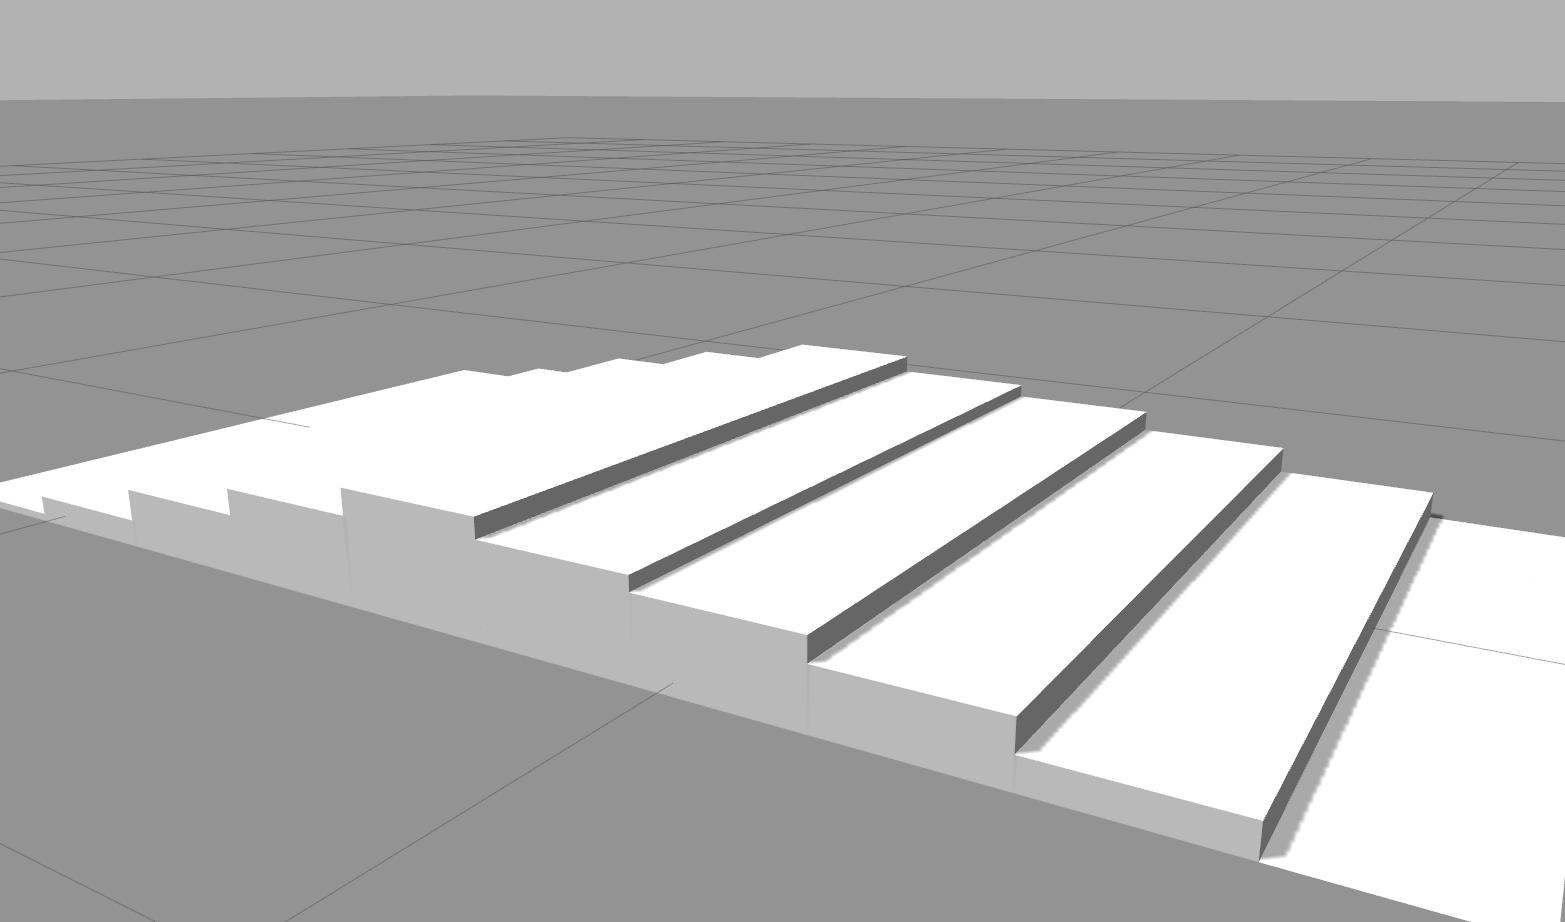
\includegraphics[height=3cm,width=2.5cm,keepaspectratio]{terrain_2.jpg}\end{minipage} & \cellcolor[HTML]{DAE8FC}10 & 68 &  \\ [0.5cm] \cline{3-4}
        \multirow{-3}{*}{\textbf{Этап 2}} & \begin{minipage}{2.5cm}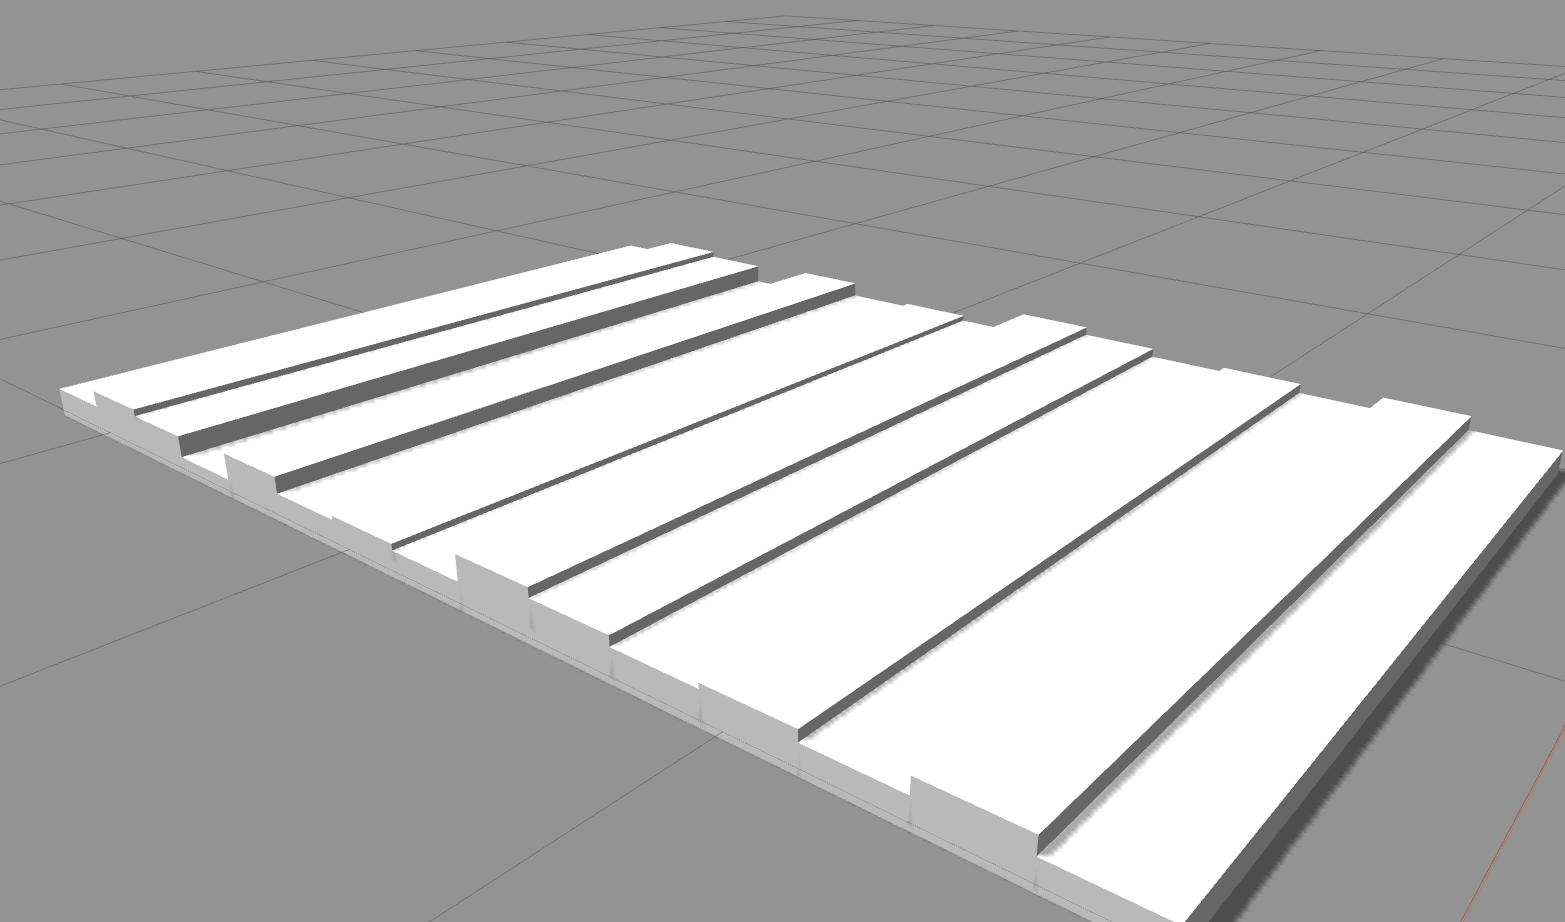
\includegraphics[height=3cm,width=2.5cm,keepaspectratio]{terrain_3.jpg}\end{minipage} & \cellcolor[HTML]{DAE8FC}12 & 77 & \multirow{-3}{*}{55}
        \end{tabular}
        % \caption*{\large\centering\textbf{Summary}: created robot should have 10-12 legs in total}
        \end{table}

\end{frame}

\begin{frame}[t]{Разработка робота}
    \framesubtitle{Закономерность}
    \begin{columns}[T,onlytextwidth]
        \begin{column}{0.49\textwidth}
            Лучшие роботы в экспериментах начинались с 8 до 14 ног для различных значений $\omega$. 
            
            Это объясняется критерием статического равновесия. В таком случае минимум 4 ноги всегда касаются поверхности.    
        \end{column}
        \begin{column}{0.49\textwidth}
            \vspace{-1.8cm}
            \begin{figure}[H]
                \centering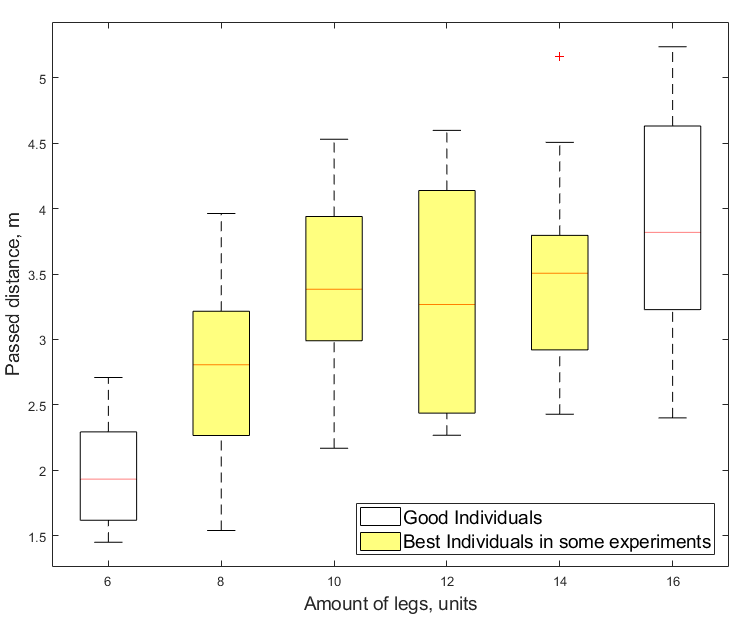
\includegraphics[height=5cm,width=1\textwidth,keepaspectratio]{box_plot_structural_synthesis.png}
                \caption*{Зависимость между кол-вом ног и пройденной дистанцией}
                \label{fig:box_plot_structural_synthesis.png}
            \end{figure}
        \end{column}
    \end{columns}
\end{frame}

\begin{frame}[t]{Разработка преобразователя силы}
    \framesubtitle{}
    {\large\begin{block}{Вопрос}
            Как получить силу реакции опоры?
        \end{block}}
    {\large\begin{alertblock}{Ответ}
        \vspace{-0.2cm}

         \begin{itemize}
            \color{lightgray}
            \item Измерив ток/напряжение на моторе
                \item Установив датчик момента на вал мотора
                \item {\color{black} Установив датчик силы на ногу робота \\  \alert{\textbf{Пьезорезистивный датчик основанный на \underline{Velostat}}: дешевый и надежный, но имеет проблемы с гистерезисом}}
            \end{itemize}
        \end{alertblock}}
\end{frame}

\begin{frame}[t]{Разработка преобразователя силы}
    \framesubtitle{Velostat}
    \vspace{-15pt}
    \begin{columns}[T,onlytextwidth]
        \begin{column}{0.6\textwidth}
                Представляет собой полимерный материал, наполненный техническим углеродом.\\
                \textbf{Встреченные проблемы}:
                \begin{itemize}
                    \item \underline{Гистерезис} -- зависимость от текущего и предыдущих состояний
                    \item \underline{Нелинейность материала}
                    \item \underline{Малая точность} при весе от 300 грамм
                    \item \underline{Разность значений при одинаковом давлении}, когда площадь нажатия меньше датчика $\rightarrow$ \alert{Научная задача -- охарактеризовать материал для таких случаев}
                \end{itemize}
        \end{column}
        \begin{column}{0.38\textwidth}
            \vspace{-1.1cm}
            \begin{figure}[H]
                \begin{subfigure}{0.9\textwidth}
                    \centering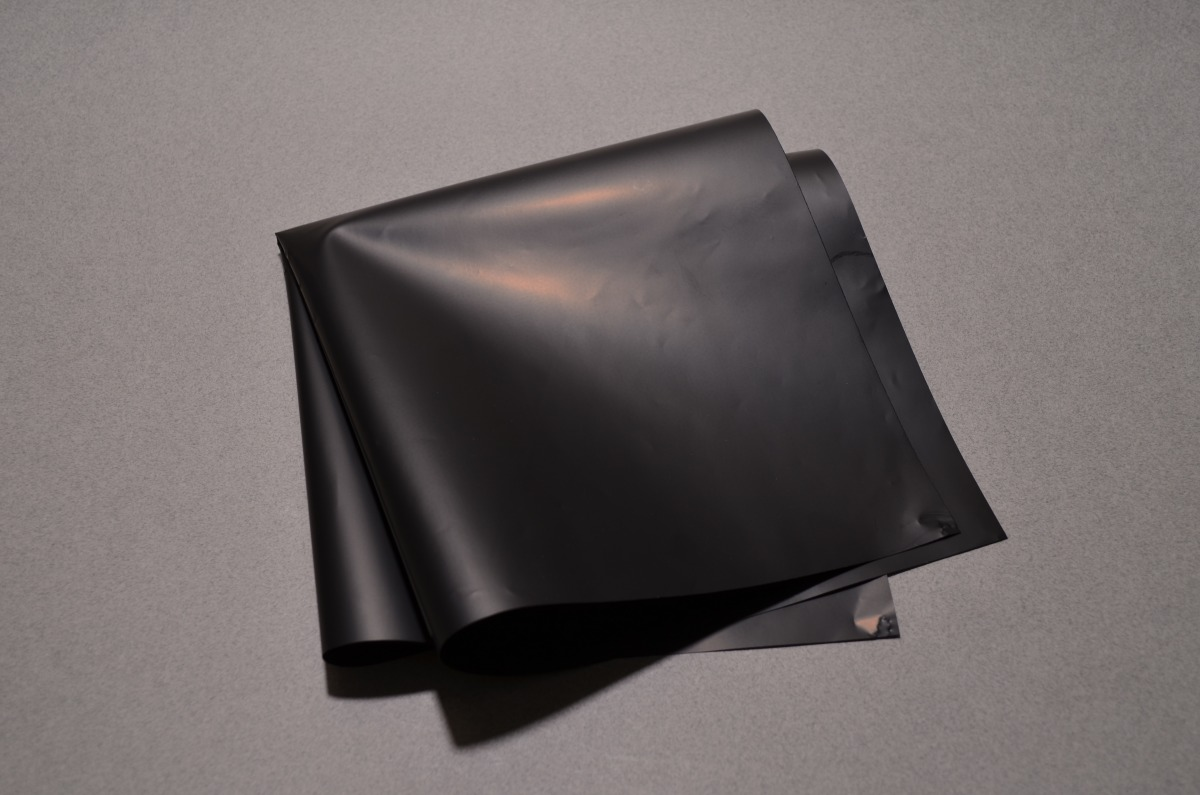
\includegraphics[height=3cm,width=1\textwidth,keepaspectratio]{velostat_sensor.jpg}
                    % \caption*{Velostat material}
                    \label{fig:velostat_sensor.jpg}
                \end{subfigure}

                \begin{subfigure}{0.9\textwidth}
                    \centering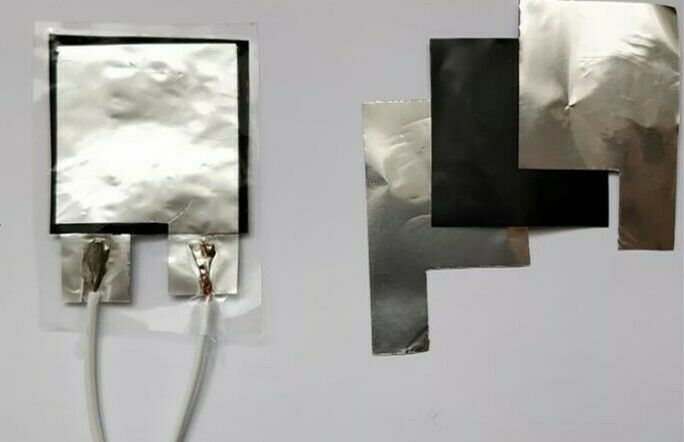
\includegraphics[height=2.9cm,width=1\textwidth,keepaspectratio]{simplest_sensor.jpg}
                    \caption*{Простейший преобразователь силы}
                    \label{fig:simplest_sensor.jpg}
                \end{subfigure}
            \end{figure}
        \end{column}
    \end{columns}

\end{frame}

\begin{frame}[t]{Разработка преобразователя силы}
    \framesubtitle{Эксперименты}
    \vspace{-15pt}
    \begin{columns}[T,onlytextwidth]
        \begin{column}{0.6\textwidth}
            {\large
                \begin{enumerate}
                    \item \textbf{Статический}. Прикладывается статический груз с размером в сенсор
                          \item\textbf{Динамический}.
                          \begin{itemize}
                            \large
                              \item Преобразователь представляется в виде сетки $4\times4$. Мы касаемся с одинаковым давлением, используя все 5 насадок
                              \item Используются насадки только 2 и 15 мм. Происходит нажатие с силой 5, 10, 20, 30, 40 H
                          \end{itemize}
                \end{enumerate}
            }
        \end{column}
        \begin{column}{0.39\textwidth}
            \vspace{-0.5cm}
            \begin{figure}[H]
                \centering
                \begin{tikzpicture}

                    % Include the image in a node
                    \node [
                        above right,
                        inner sep=0] (image) at (0,0) {\centering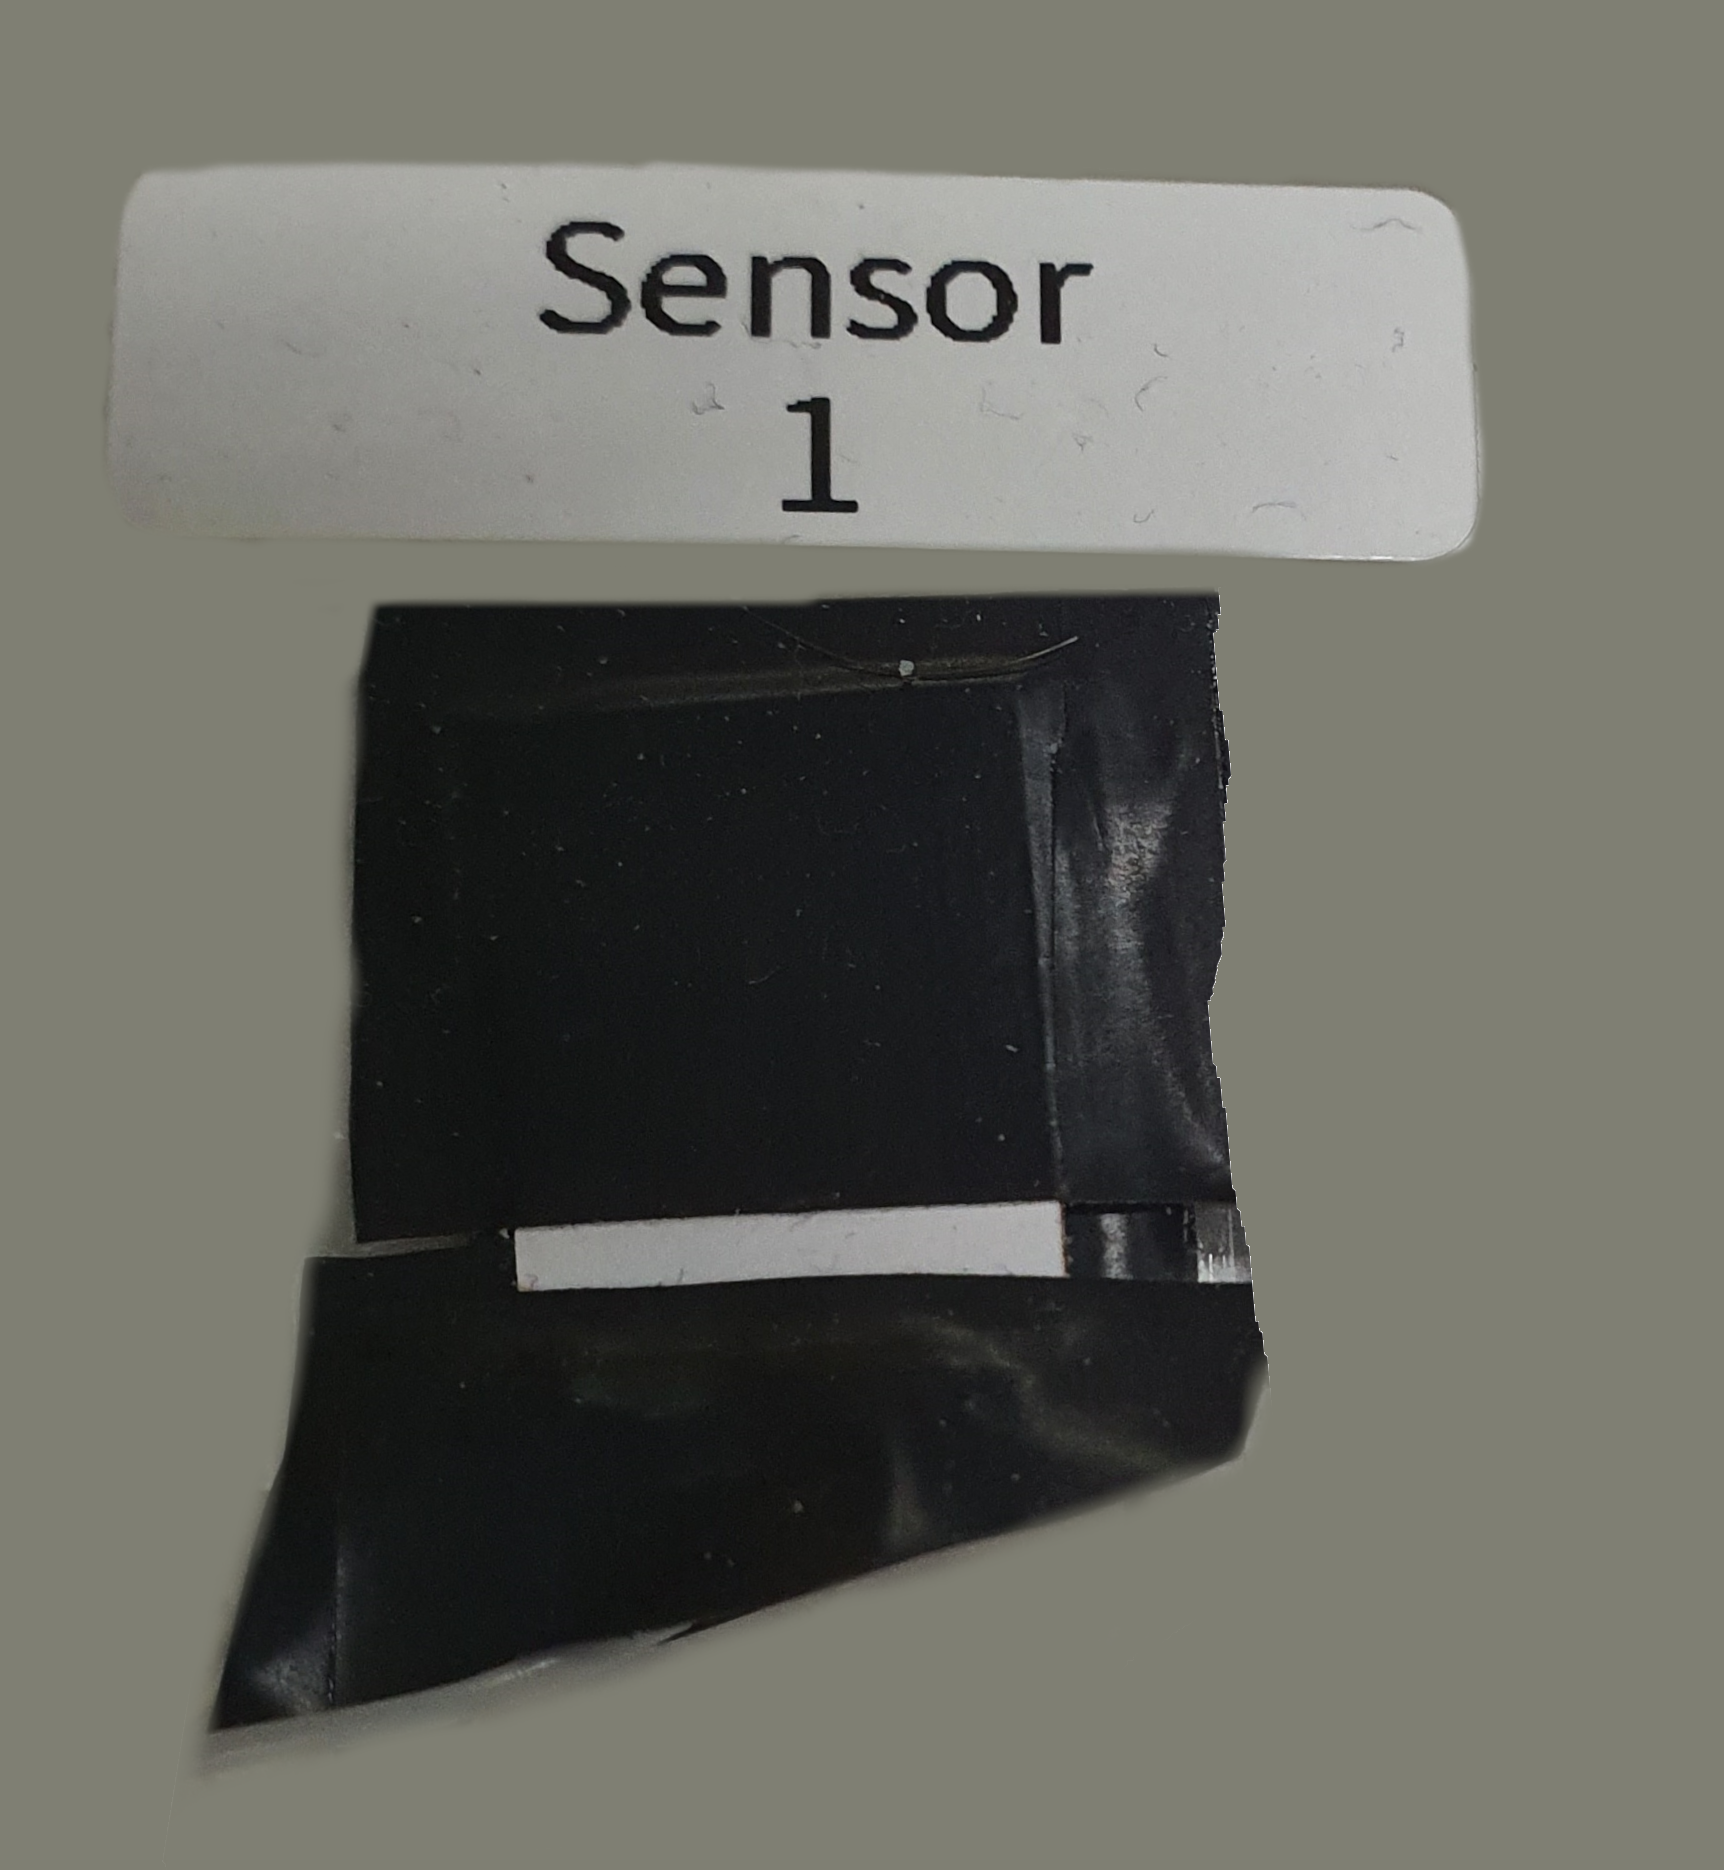
\includegraphics[height=5cm,width=1\textwidth,keepaspectratio]{sensors_grid.png}};

                    % Create scope with normalized axes
                    \begin{scope}[
                            x={($0.1*(image.south east)$)},
                            y={($0.1*(image.north west)$)}]

                        % Grid
                        % \draw[lightgray,step=1] (image.south west) grid (image.north east);

                        % % Axes' labels
                        % \foreach \x in {0,1,...,10} { \node [below] at (\x,0) {\x}; }
                        % \foreach \y in {0,1,...,10} { \node [left] at (0,\y) {\y};}

                        % Labels
                        % Simple brace
                        \draw [green, very thick,
                            decorate,
                            decoration = {brace,
                                    raise=5pt,
                                    amplitude=5pt,
                                    aspect=0.5}] (6,3.7) --  (3,3.7)
                        node[pos=0.5,below=10pt,green]{$15\ mm$};

                        \draw [green, very thick,
                            decorate,
                            decoration = {brace, mirror,
                                    raise=5pt,
                                    amplitude=5pt,
                                    aspect=0.5}] (6,3.6) --  (6,6.4)
                        node[pos=0.5,right=10pt,green]{$15\ mm$};

                        \draw[green,step=1,xshift=34, yshift=43]  (0.5,0.5) grid +(3,3);

                        \node[circle,fill=green,scale=0.4] at (3.3,6.27){\small 1};
                        \node[circle,fill=green,scale=0.4] at (5.92,3.7){\small 16};
                    \end{scope}

                \end{tikzpicture}
                \caption*{Представление сенсора \\ как $4\times4$ сетки}
                \label{fig:file_name}
            \end{figure}
        \end{column}
    \end{columns}
\end{frame}

\begin{frame}[t]{Разработка преобразователя силы}
    \framesubtitle{Результаты: Статический эксперимент}
    \vspace{-0.5cm}
    \begin{columns}[T,onlytextwidth]
        \begin{column}{0.52\textwidth}
            \begin{eqnarray*}
                V_{out} = V_0 + p[k_p + k_e(1-e^\frac{-(t-t_0)}{\tau_{res}})](1-e^{-\frac{A}{p}}) \\
                k_p = A_1e^{-A_2p}; \tau_{res} = B_0 + B_1e^{-\frac{p}{B_2}}
            \end{eqnarray*}
            Где $V_0$ -- начальное напряжение, \\ $p$ -- приложенное давление, \\ $A_i,\ B_i,\ \tau_{res},\ k_i$ искомые параметры, \\  $t$ -- текущее время, $t_0$ -- время начала нажатия. 
            \\ \alert{Апробированна модель для калибровки датчика}
        \end{column}
        \begin{column}{0.45\textwidth}
            \vspace{-15pt}
            \begin{figure}[H]
                \begin{subfigure}{0.99\textwidth}
                    \centering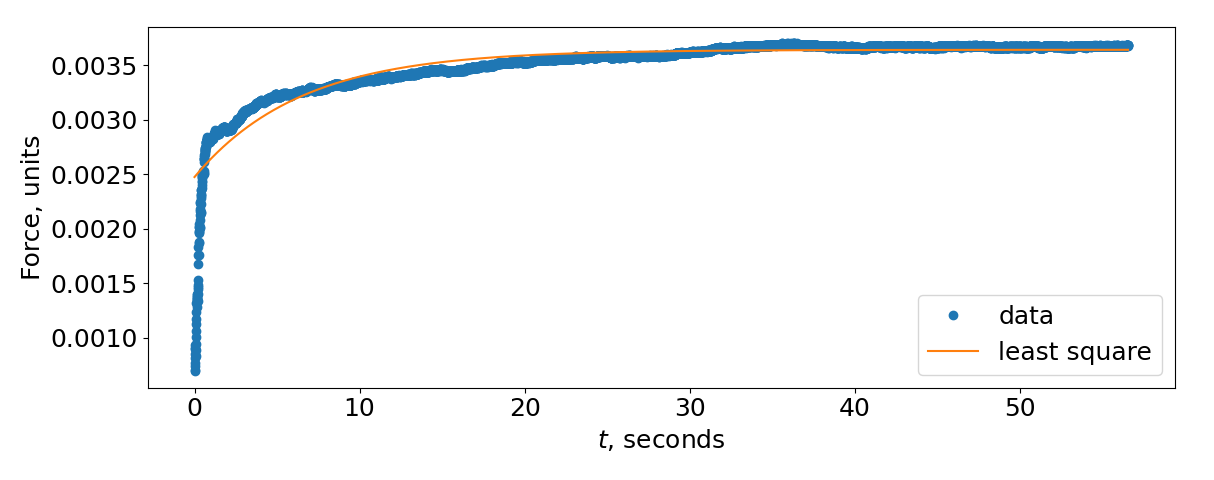
\includegraphics[height=2.8cm,width=1\textwidth,keepaspectratio]{least_square_model.png}
                    \label{fig:least_square_model.png}
                \end{subfigure}
                \vspace{-1cm}

                \begin{subfigure}{0.99\textwidth}
                        \centering
                         \begin{tikzpicture}
                            % Include the image in a node
                            \node [above right, inner sep=0] (image) at (0,0) 
                            {\centering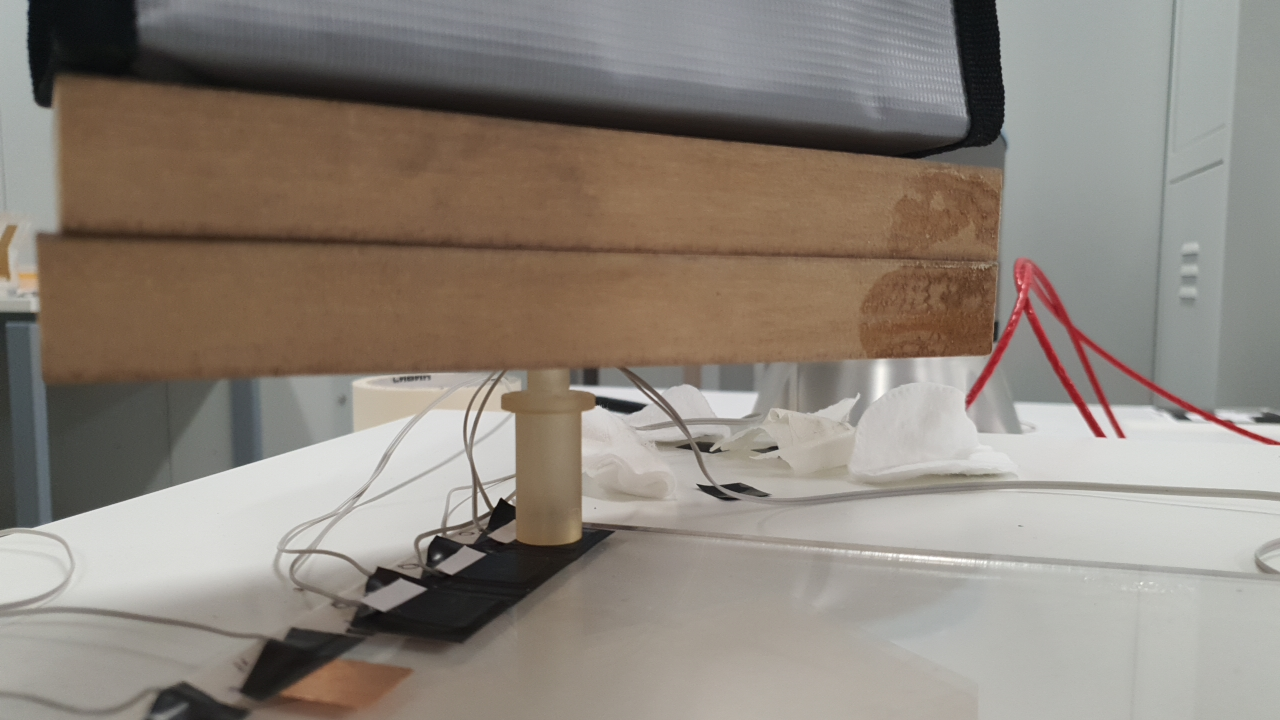
\includegraphics[height=3.4cm,width=1\textwidth,keepaspectratio]{static_load_meh.JPG}};          
                            % Create scope with normalized axes
                            \begin{scope}[
                                x={($ 0.1*(image.south east)$)},
                                y={($ 0.1*(image.north west)$)}]
                                % Grid and axes' labels
                                % \draw[lightgray,step=1] (image.south west) grid (image.north east);
                                % \foreach \x in {0,1,...,10} { \node [below] at (\x,0) {\x}; }
                                % \foreach \y in {0,1,...,10} { \node [left] at (0,\y) {\y};}
                                % Labels
                            \draw[latex-, very thick,green] (4.3,2.3) -- (5,1.6)
                                node[rounded corners=3pt,below right,black,fill=white]{\tiny Velostat sensor};
                            
                            \draw[latex-, very thick,green] (4.3,3.5) -- (5.5,2.45)
                                node[rounded corners=3pt,right,black,fill=white]{\tiny \O \ 15 mm end-effector};

                            \draw[latex-, very thick,green] (6,6) -- (6.4,4.9)
                                node[rounded corners=3pt,below right,black,fill=white]{\tiny Known static load};
                            \end{scope}
                        \end{tikzpicture}
                        % \caption*{}
                \end{subfigure}
            \end{figure}
        \end{column}
    \end{columns}
\end{frame}

\begin{frame}[t]{Разработка преобразователя силы}
    \framesubtitle{Требования к установке}
    \vspace{-0.5cm}
    \begin{columns}[T,onlytextwidth]
        \begin{column}{0.39\textwidth}
            \begin{itemize}
                \item Управление силой нажатия {\\ \alert{Импедансное управления}}
                \item Повторяемость эксперимента по силе и позиции{\\ \alert{Добавив манипулятор и камеру}}
                \item Возможность нажимать только на часть сенсора{\\ \alert{Насадки для манипулятора}}
            \end{itemize}
        \end{column}
        \begin{column}{0.8\textwidth}
            \scalebox{0.81}{
            \begin{tikzpicture}

                % Include the image in a node
                \node [
                    above right,
                    inner sep=0] (image) at (0,0) {\centering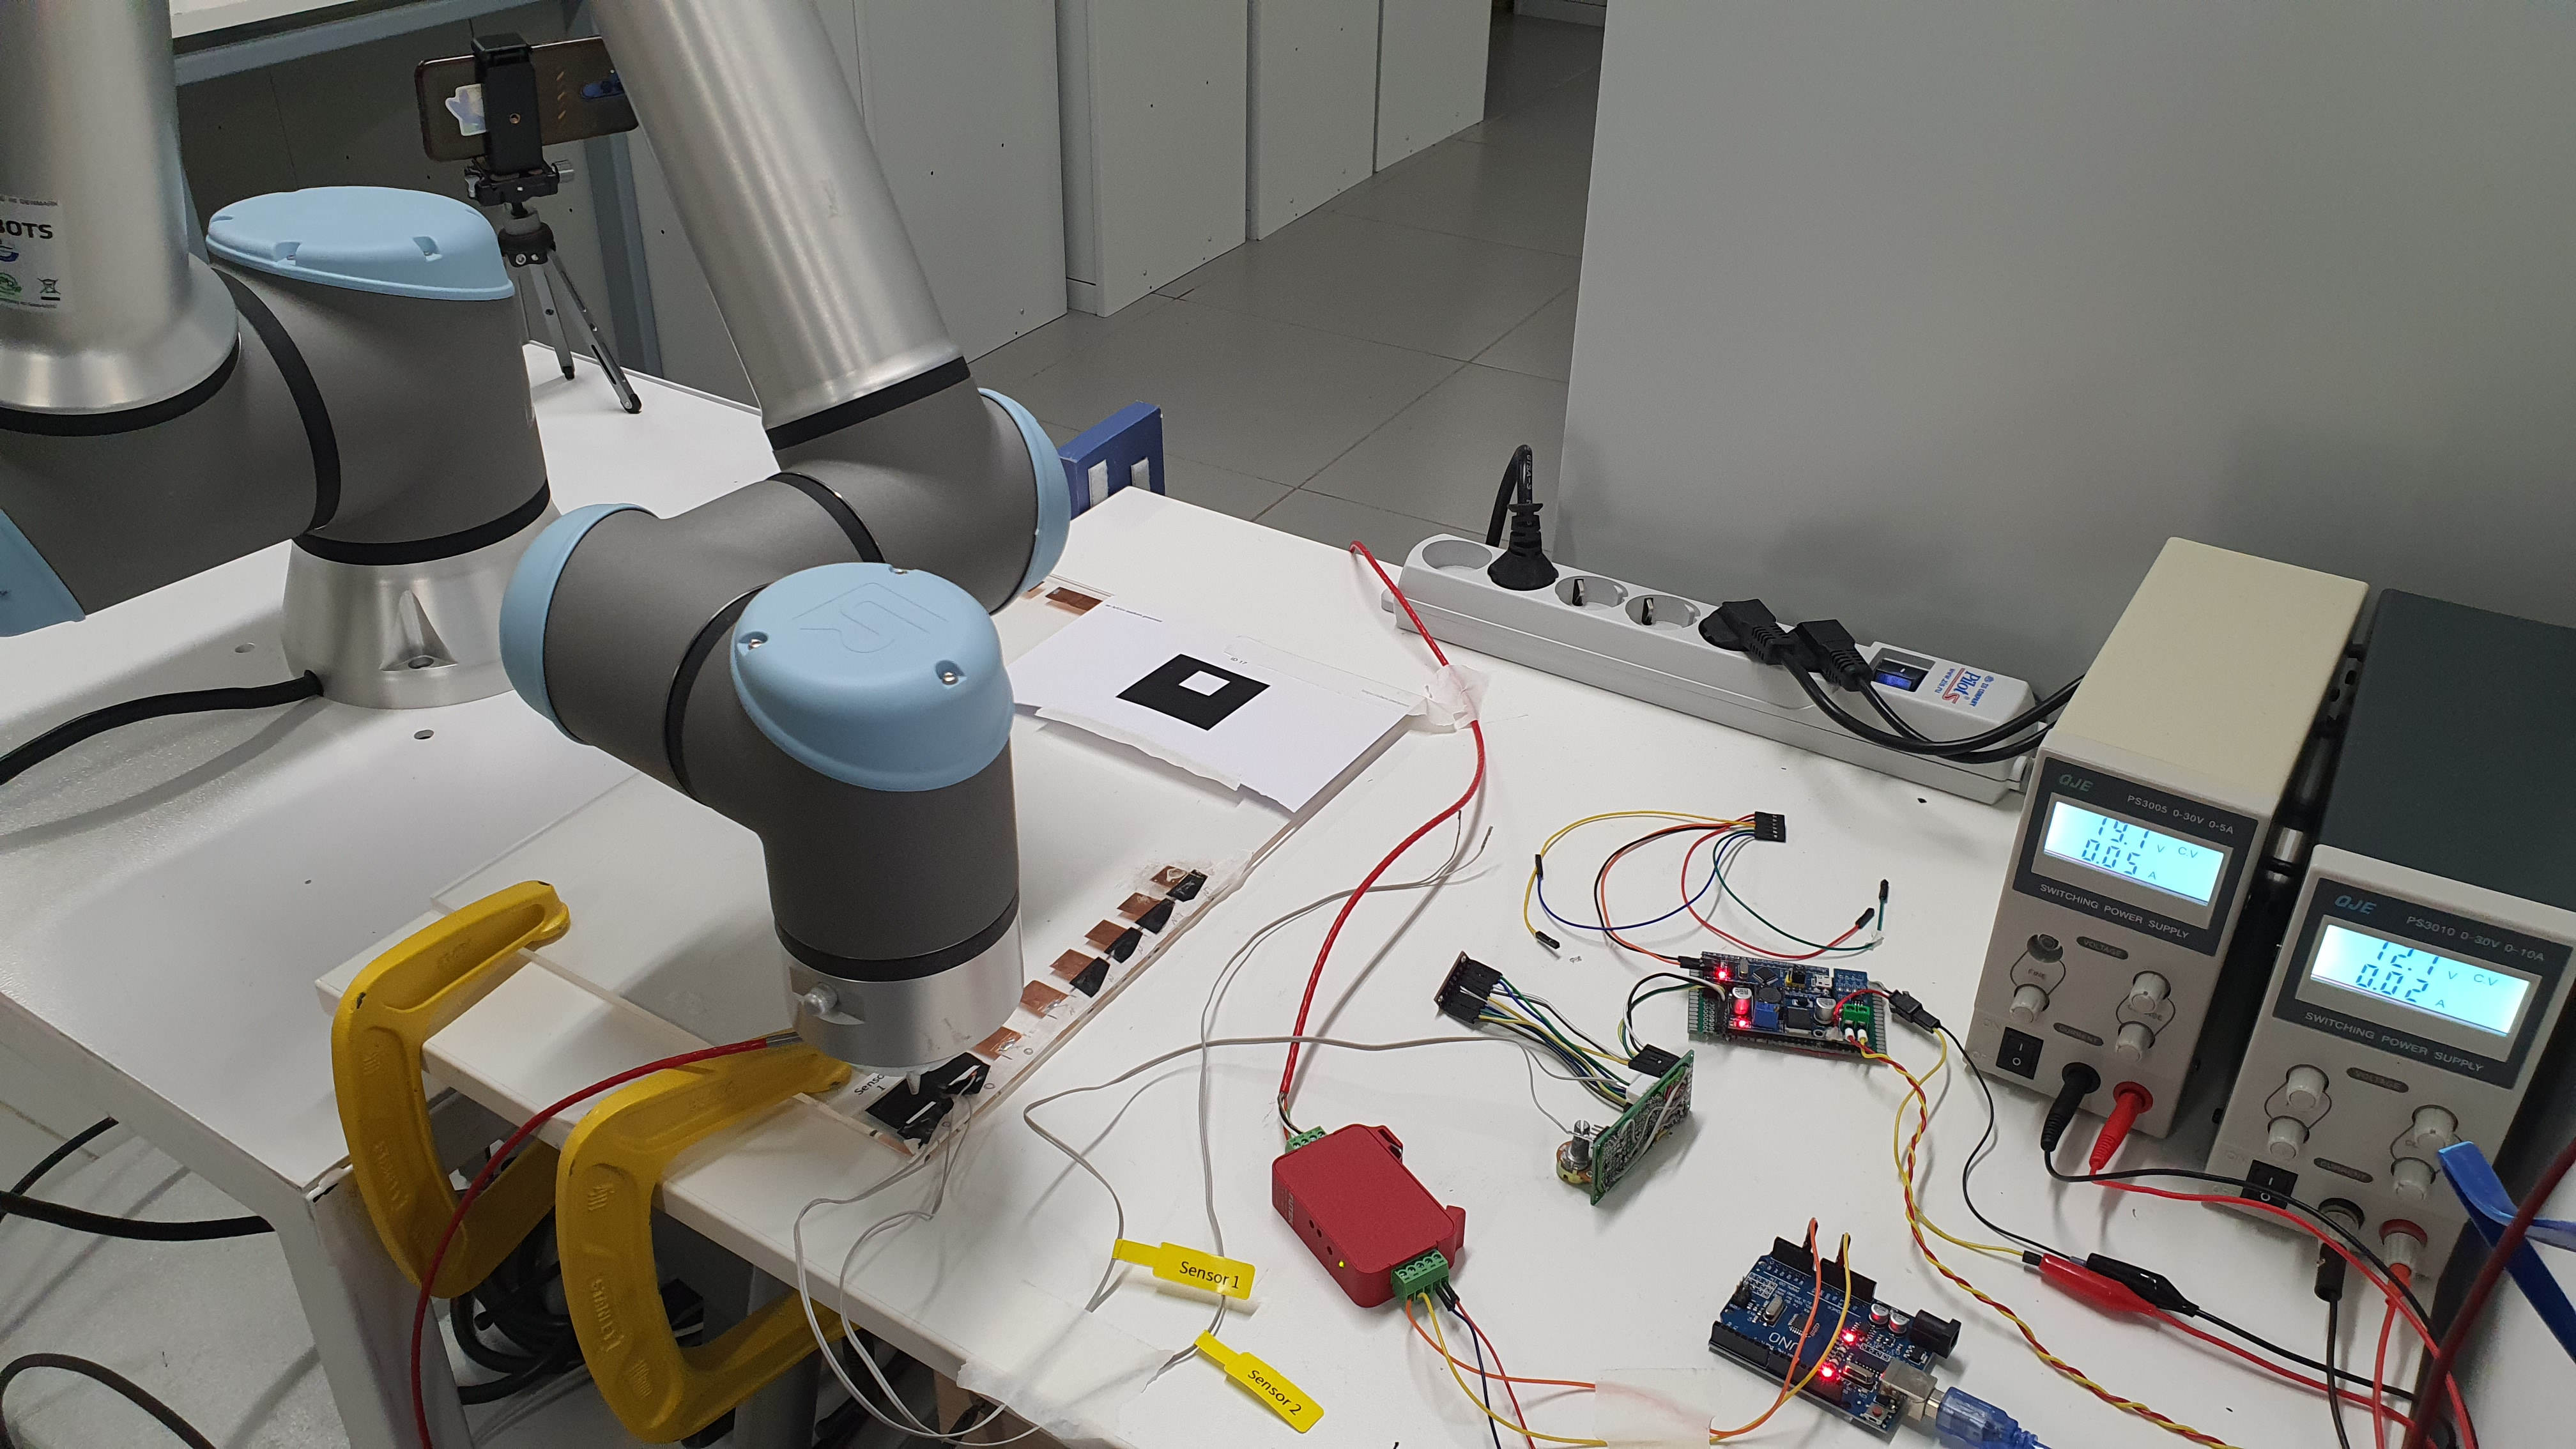
\includegraphics[height=6cm,width=1\textwidth,keepaspectratio]{exp_stand1}};
    
                % Create scope with normalized axes
                \begin{scope}[
                        x={($0.1*(image.south east)$)},
                        y={($0.1*(image.north west)$)}]
    
                    % Grid
                    % \draw[lightgray,step=1] (image.south west) grid (image.north east);
    
                    % % Axes' labels
                    % \foreach \x in {0,1,...,10} { \node [below] at (\x,0) {\x}; }
                    % \foreach \y in {0,1,...,10} { \node [left] at (0,\y) {\y};}
    
                    % Labels
                    % \node[circle,fill=green] at (7.25,6.75){\small 2};
    
                    \draw[latex-, very thick,green] (3.5,2.2) -- (2.5,1)
                    node[rounded corners=3pt,below left,black,fill=white]{\small Velostat sensors};
    
                    \draw[stealth-, very thick,green] (3.5,2.6) -- ++(-0.7,+0.5)
                    node[rounded corners=3pt,left,black,fill=white]{\small Force sensor};
    
                    \draw[stealth-, very thick,green] (6.5,3) -- (7,6)
                    node[rounded corners=3pt,above right,black,fill=white]{\small Self-made PCB};
    
                    \draw[stealth-, very thick,green] (7.2,1.5) -- (8,5)
                    node[rounded corners=3pt,above right,black,fill=white]{\small Arduino};
    
                    \draw[stealth-, very thick,green] (2.5,9.5) -- (4,9.5)
                    node[rounded corners=3pt,right,black,fill=white]{\small Camera};
    
                    \draw[very thick,green] (0.5,2.5) rectangle (4.2,9)
                    node[below left,black,fill=green]{\small UR10e};
    
                    \draw[latex-, very thick,green] (4.5,7.2) edge (5.5,7.5)
                    (4.8,5.3) -- (5.5,7.5)
                    node[rounded corners=3pt,above,black,fill=white]{\small Aruco markers};
                \end{scope}
    
            \end{tikzpicture}
            }
        \end{column}
    \end{columns}

\end{frame}

\begin{frame}[t]{Разработка преобразователя силы}
    \framesubtitle{Установка: Насадки}
    \vspace{-0.9cm}
    \begin{columns}[T,onlytextwidth]
        \begin{column}{0.6\textwidth}
            \begin{figure}[H]
                \centering
                \begin{tikzpicture}
                    % Include the image in a node
                    \node [above right, inner sep=0] (image) at (0,0)
                    {\centering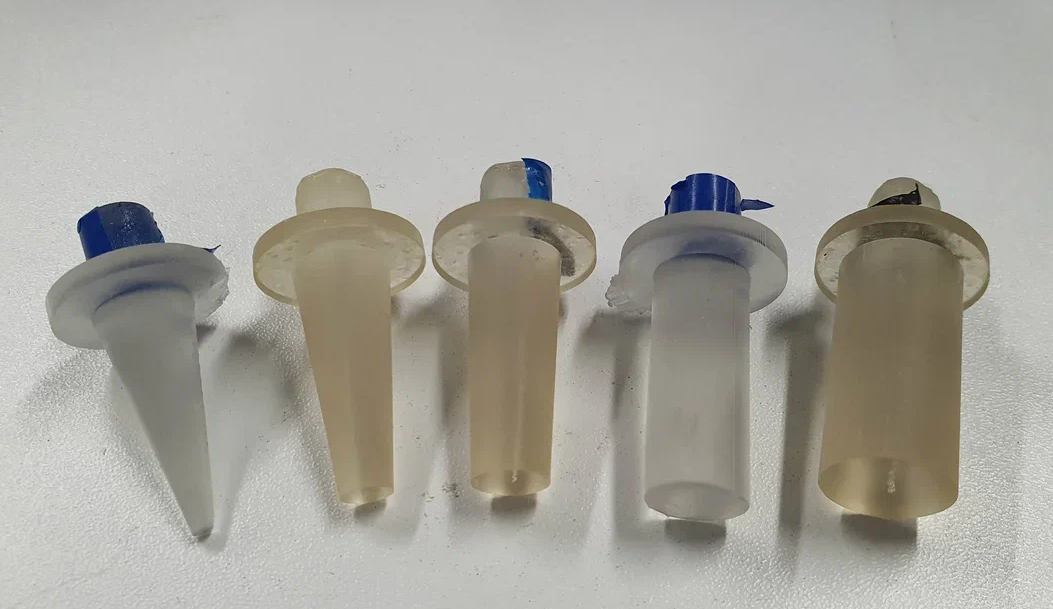
\includegraphics[height=5cm,width=1\textwidth,keepaspectratio]{all_end_effectors.png}};
                    % Create scope with normalized axes
                    \begin{scope}[
                            x={($ 0.1*(image.south east)$)},
                            y={($ 0.1*(image.north west)$)}]
                        % Grid and axes' labels
                        % \draw[lightgray,step=1] (image.south west) grid (image.north east);
                        % \foreach \x in {0,1,...,10} { \node [below] at (\x,0) {\x}; }
                        % \foreach \y in {0,1,...,10} { \node [left] at (0,\y) {\y};}

                        % Labels
                        \node[rounded corners=3pt,black,fill=white] at (1.1,7.4){\tiny 2 mm };
                        \node[rounded corners=3pt,black,fill=white] at (3.1,7.9){\tiny 6 mm };
                        \node[rounded corners=3pt,black,fill=white] at (4.9,8.1){\tiny 8 mm };
                        \node[rounded corners=3pt,black,fill=white] at (6.7,7.9){\tiny 12 mm };
                        \node[rounded corners=3pt,black,fill=white] at (8.6,7.9){\tiny 15 mm };
                    \end{scope}
                \end{tikzpicture}
                \caption*{Все насадки}
                \label{fig:all_end_effectors.png}
            \end{figure}
        \end{column}
        \begin{column}{0.39\textwidth}
            \vspace{-1.3cm}

            \begin{figure}[H]
                \begin{subfigure}[t]{0.6\textwidth}
                    \centering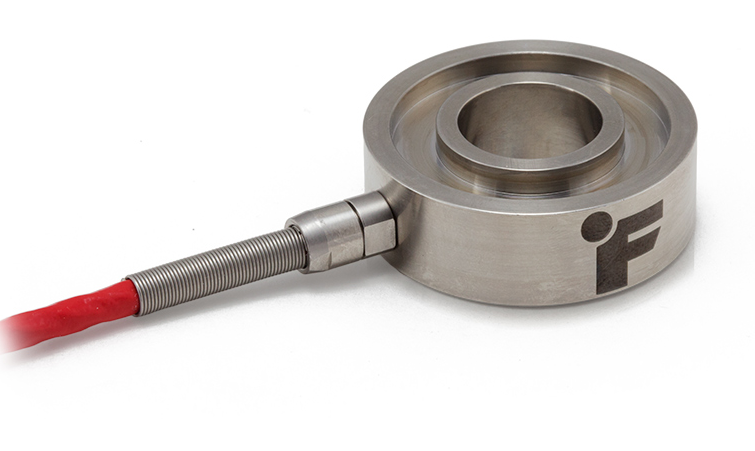
\includegraphics[width=0.99\textwidth]{LTH350-DONUT-LOAD-CELL-1.png}\\
                    \caption*{\normalsize Промышленный \\ датчик силы}
                    \label{fig:futek}
                \end{subfigure}
                \vspace{-0.2cm}

                \begin{subfigure}[t]{0.6\textwidth}
                    \centering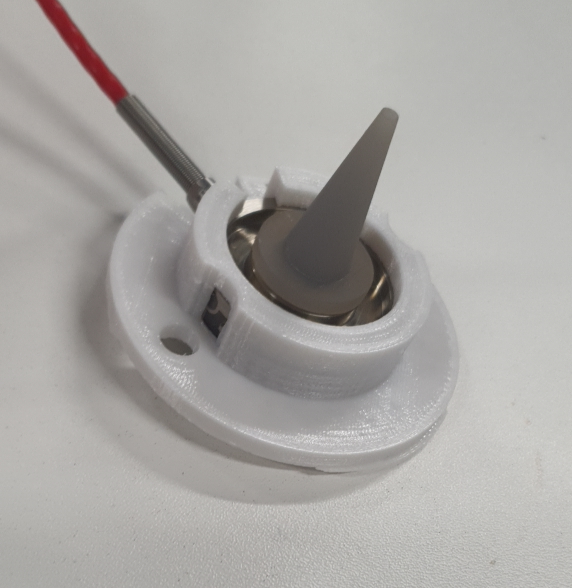
\includegraphics[width=0.99\textwidth]{point_load.JPG}\\
                    \caption*{\normalsize Насадка в сборке}
                    \label{fig:point_load}
                \end{subfigure}
            \end{figure}

        \end{column}
    \end{columns}
\end{frame}

\begin{frame}[t]{Разработка преобразователя силы}
    \framesubtitle{Установка: Видео}
    \vspace{-15pt}
    \begin{figure}[H]
        % \href{run:./videos/exp_stand_video.mp4}{
        \href{https://youtu.be/Gw4wVZ-ESuE}{
            \centering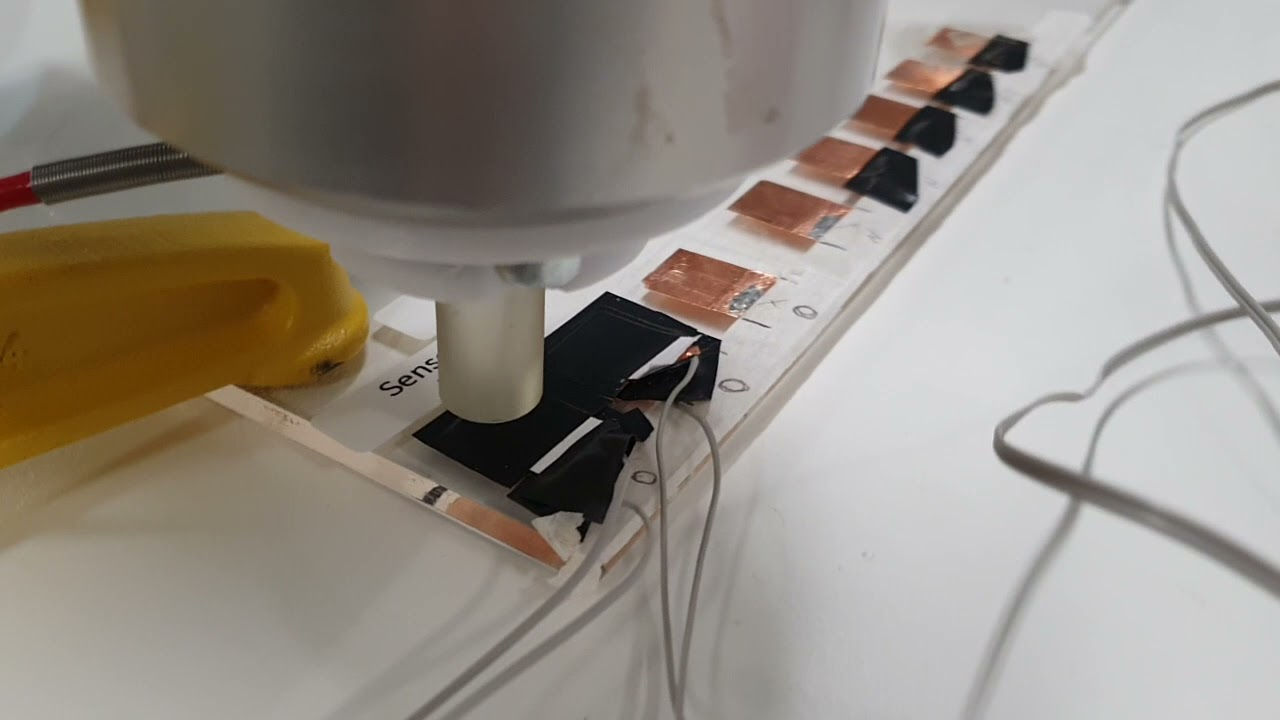
\includegraphics[height=6cm,width=1\textwidth,keepaspectratio]{exp_stand_video_preview.jpg}}
        % \caption{caption_name}
    \end{figure}
\end{frame}



\begin{frame}[t]{Разработка преобразователя силы}
    \framesubtitle{Результаты: Динамический эксперимент}
    \vspace{-15pt}
    \begin{figure}[H]
        \begin{subfigure}{0.64\textwidth}
            \centering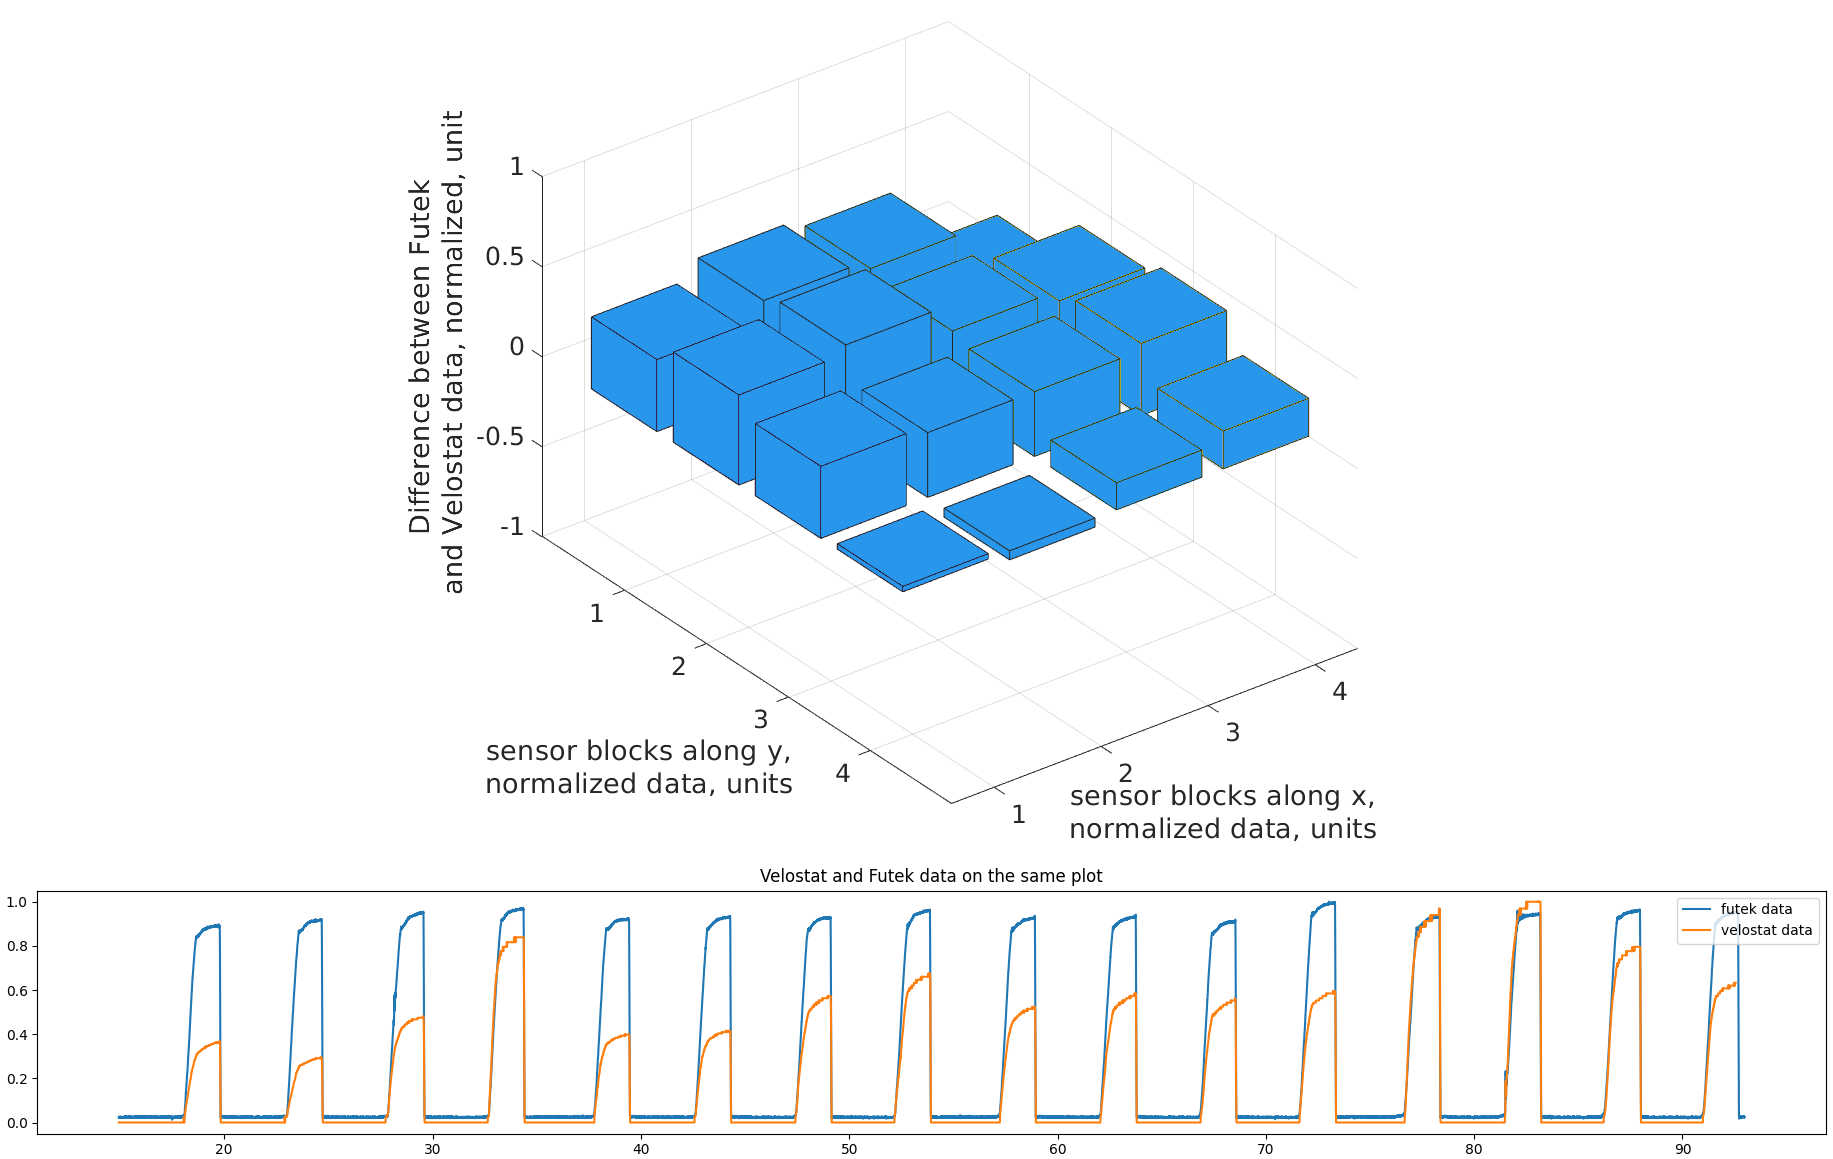
\includegraphics[height=5cm,width=1\textwidth,keepaspectratio]{sens1_pike1_mod.png}
            \caption*{2 мм диаметр насадки}
            \label{fig:sens1_pike1}
        \end{subfigure}
        \begin{subfigure}{0.34\textwidth}
            \centering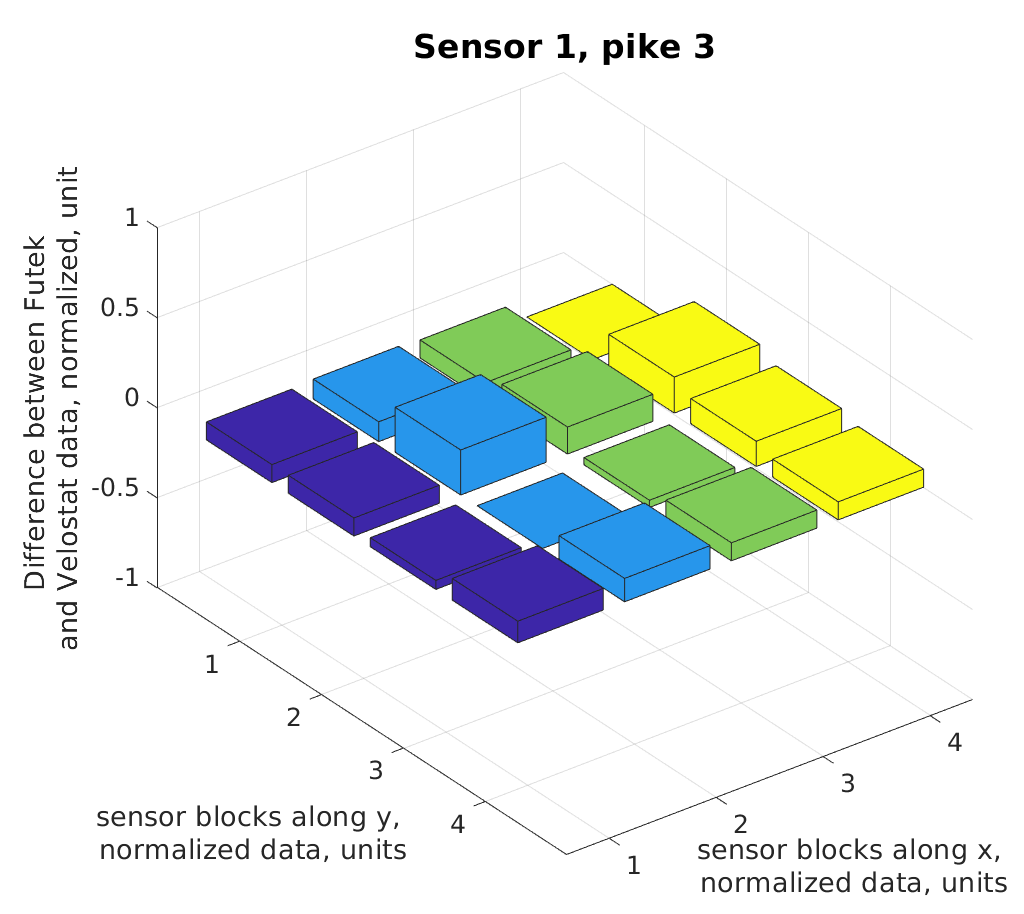
\includegraphics[height=5cm,width=1\textwidth,keepaspectratio]{sens1_pike3.png}
            \caption*{8 мм диаметр насадки}
            \label{fig:sens1_pike3}
        \end{subfigure}
    \end{figure}
    \vspace{-0.8cm}
    \alert{Одинаковые данные, когда площадь нажатия превышает 50\% от площади датчика}
\end{frame}

\begin{frame}[t]{Определение физических свойств поверхности}
    \framesubtitle{}
    \vspace{-0.3cm}
    {\large\begin{block}{Вопрос}
        Как определить тип местности во время движения по такой местности?
        \end{block}}
    {\large\begin{alertblock}{Ответ}
        1. Подготовить для экспериментов различные поверхности.

        2. Собрать датасет, состоящий из угловой скорости мотора и показаний датчиков с ног робота.

        3. Представить их в виде вектора фич.

        4. Решить задачу классификации данных с помощью SVM, используя метрику 10-fold cross validation. 

        5. Протестировать модель на собранных данных.
        \end{alertblock}}
\end{frame}

\begin{frame}[t]{Определение физических свойств поверхности}
    \framesubtitle{Требования к установке}
    \vspace{-0.5cm}
    \begin{columns}[T,onlytextwidth]
        \begin{column}{0.57\textwidth}
            \begin{itemize}
                \item Иметь возможность быстро менять используемые поверхности {\\ \alert{Быстроразборный стол}}
                \item Бесконечное движение робота {\\ \alert{2-ух степенной механизм и нога S-образной формы}}
                \item Узел движителя должен быть такой же как на СтриРусе {\\ \alert{Создано крепление для узла ноги робота}}
            \end{itemize}
        \end{column}
        \begin{column}{0.42\textwidth}
            \vspace{-0.8cm}
            \begin{figure}[H]
                \centering
                \begin{tikzpicture}
                    % Include the image in a node
                    \node [above right, inner sep=0] (image) at (0,0)
                    {\centering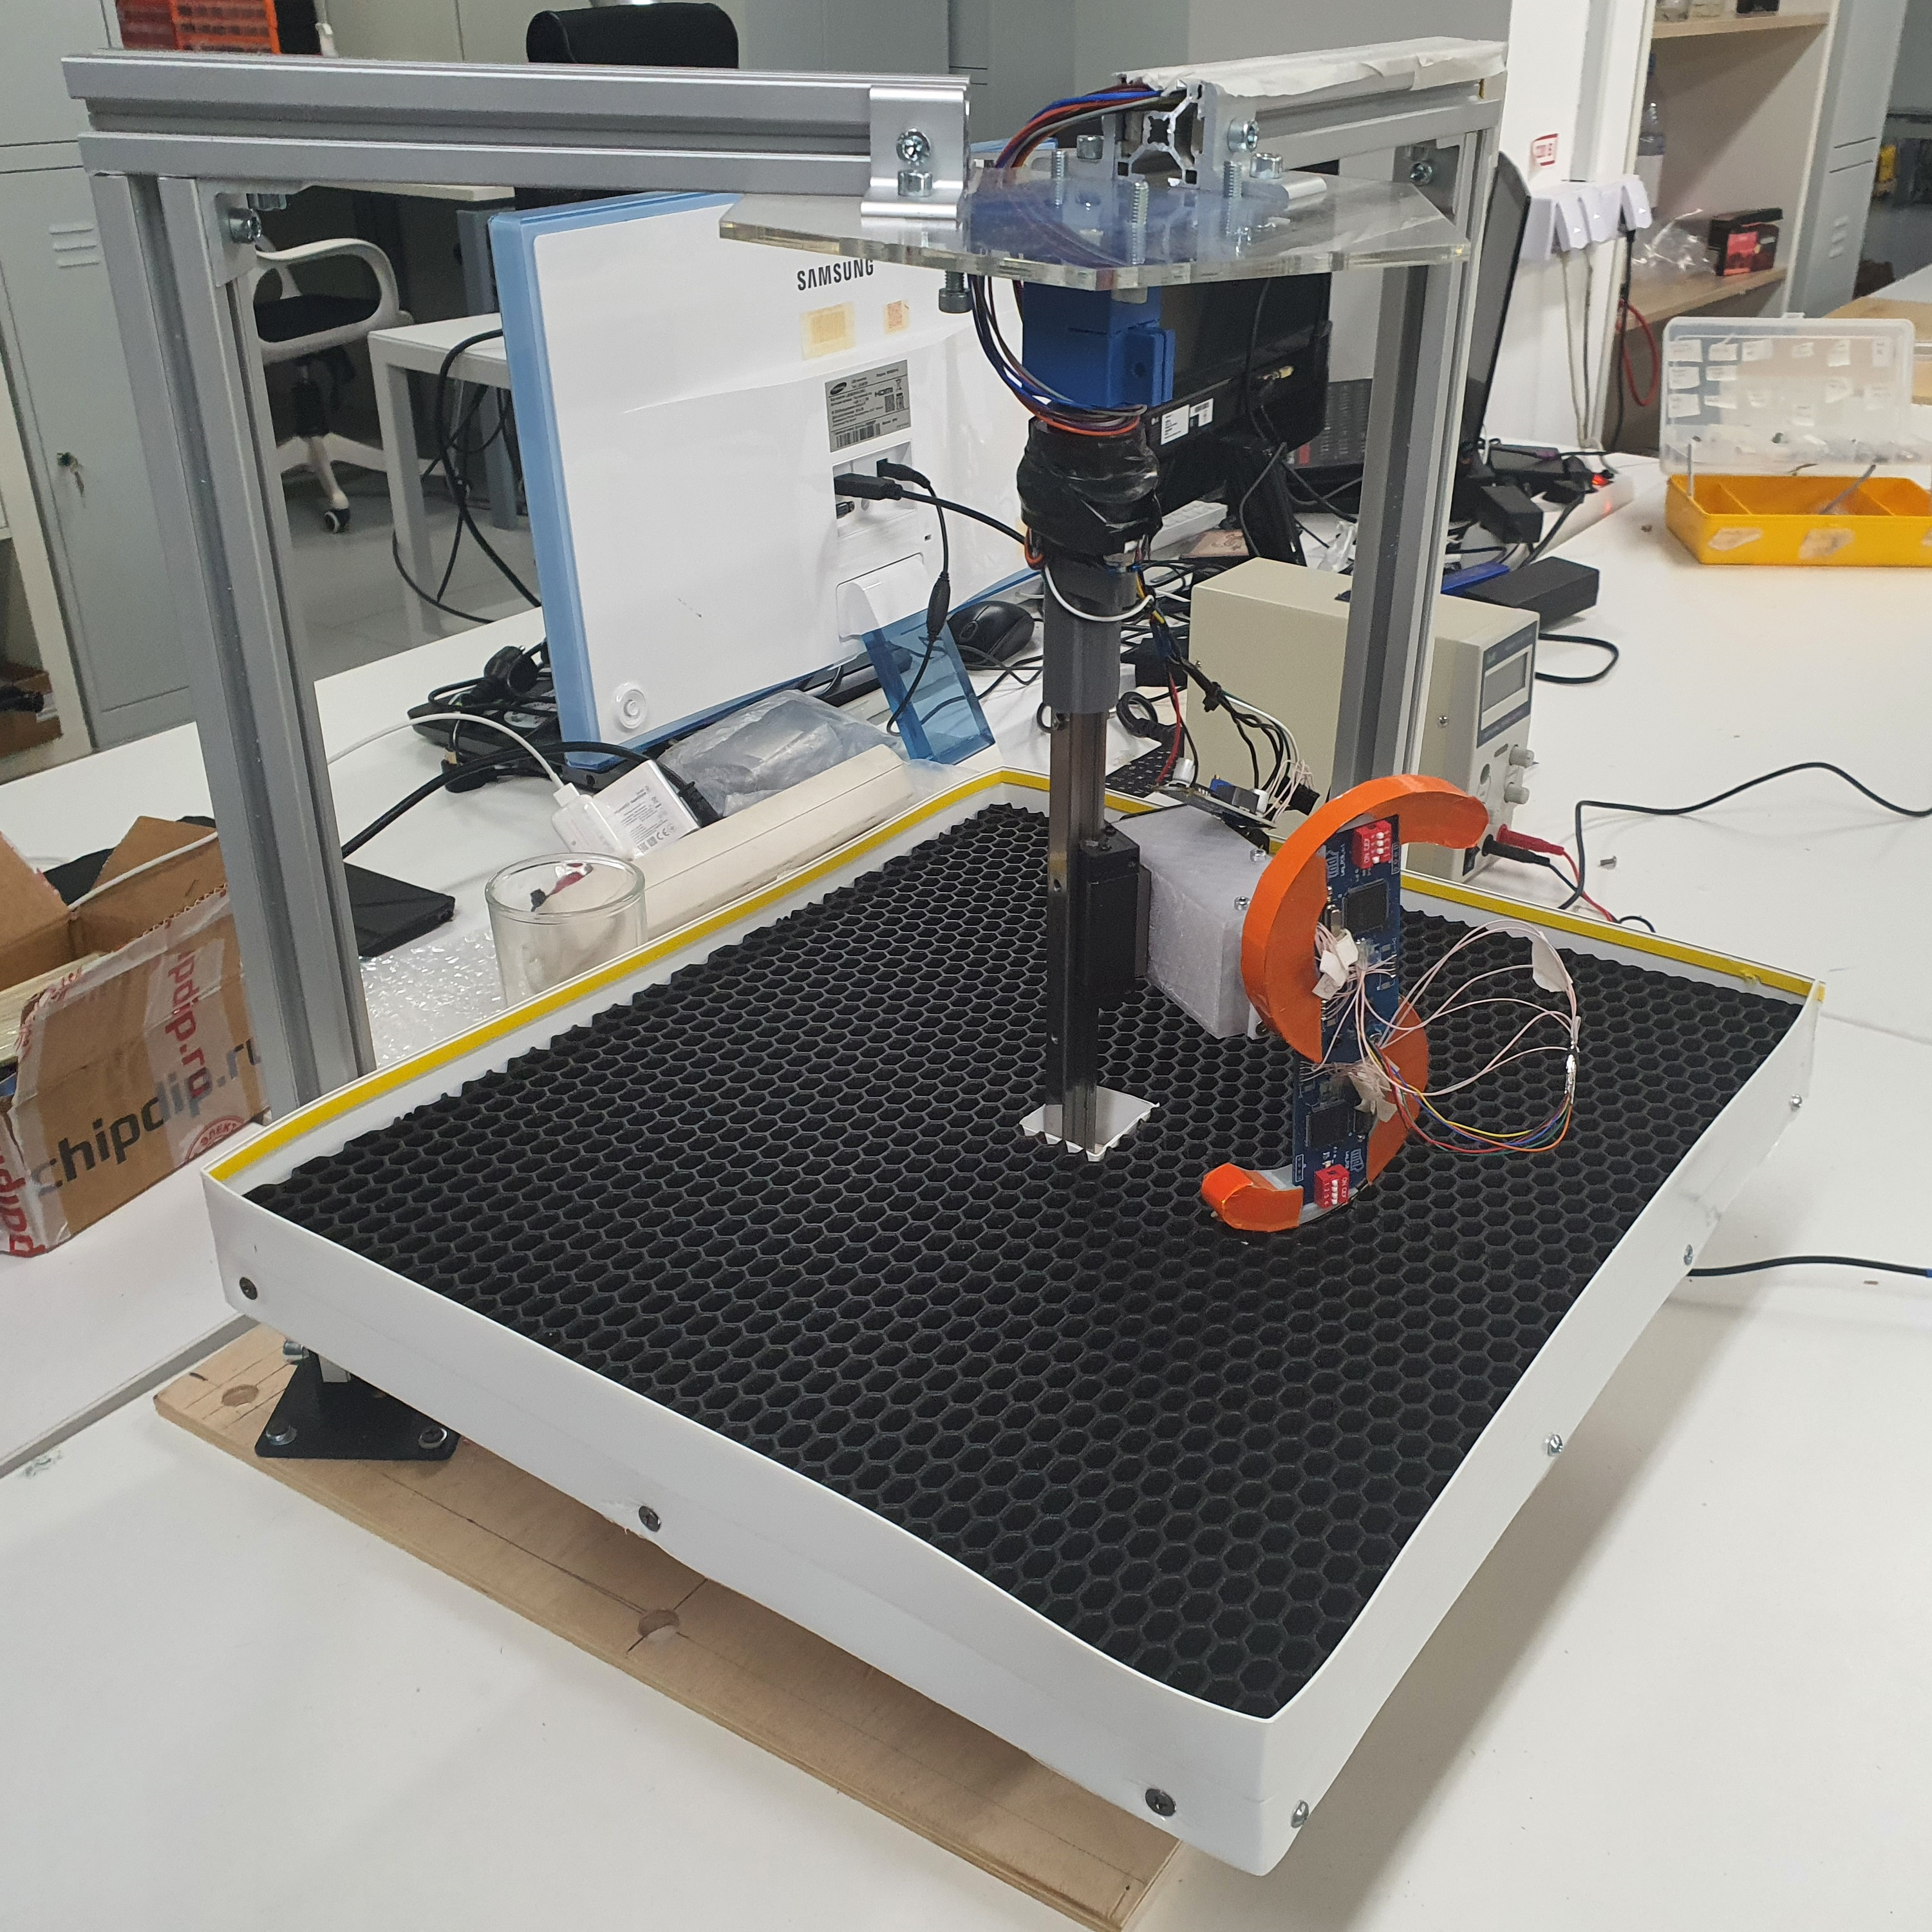
\includegraphics[height=6cm,width=1\textwidth,keepaspectratio]{s_shape_leg/s_leg_setup.JPG}};
                    % Create scope with normalized axes
                    \begin{scope}[
                            x={($ 0.1*(image.south east)$)},
                            y={($ 0.1*(image.north west)$)}]
                        % Grid and axes' labels
                        % \draw[lightgray,step=1] (image.south west) grid (image.north east);
                        % \foreach \x in {0,1,...,10} { \node [below] at (\x,0) {\x}; }
                        % \foreach \y in {0,1,...,10} { \node [left] at (0,\y) {\y};}

                        % Labels

                        % \node[circle,fill=green,scale=0.4] at (3.3,6.27){\small 1};

                        % \draw[latex-, very thick,green] (3.5,2.2) -- (2.5,1)
                        % node[below left,black,fill=white]{\small test};

                        \draw[stealth-, very thick,green] (3.5,2.5) -- (3,1.5)
                        node[rounded corners=3pt,below,black,fill=white]{\tiny Table for surfaces};

                        \draw[stealth-, very thick,green] (7.1,5.4) -- (7.4,7)
                        node[rounded corners=3pt,above right,black,fill=white]{\tiny Self-made PCB};

                        \draw[very thick,green] (6,6.1) rectangle (8.5,3.5)
                        node[above left,black,fill=green]{\tiny S leg};
                    \end{scope}
                \end{tikzpicture}
                % \caption*{}
                \label{fig:s_shape_leg/s_leg_setup.JPG}
            \end{figure}
        \end{column}
    \end{columns}
\end{frame}


\begin{frame}[t]{Определение физических свойств поверхности}
    \framesubtitle{Установка: Типы поверхности, видео}
    \vspace{-15pt}
    \begin{figure}[H]
        \begin{subfigure}{0.22\textwidth}
            % \href{run:./videos/flat.gif}
            \href{https://gifyu.com/image/SxatY}
            {\centering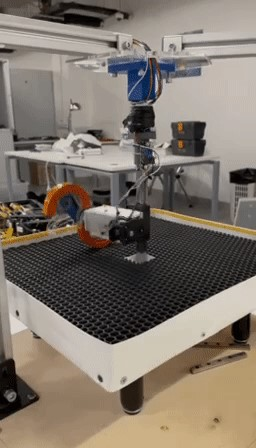
\includegraphics[height=6cm,width=1\textwidth,keepaspectratio]{s_shape_leg/flat.jpg}} 
            \caption*{Резина}
        \end{subfigure}
        \hfill
        \begin{subfigure}{0.26\textwidth}
            % \href{run:./videos/rock.gif}
            \href{https://gifyu.com/image/Sxatt}
            {\centering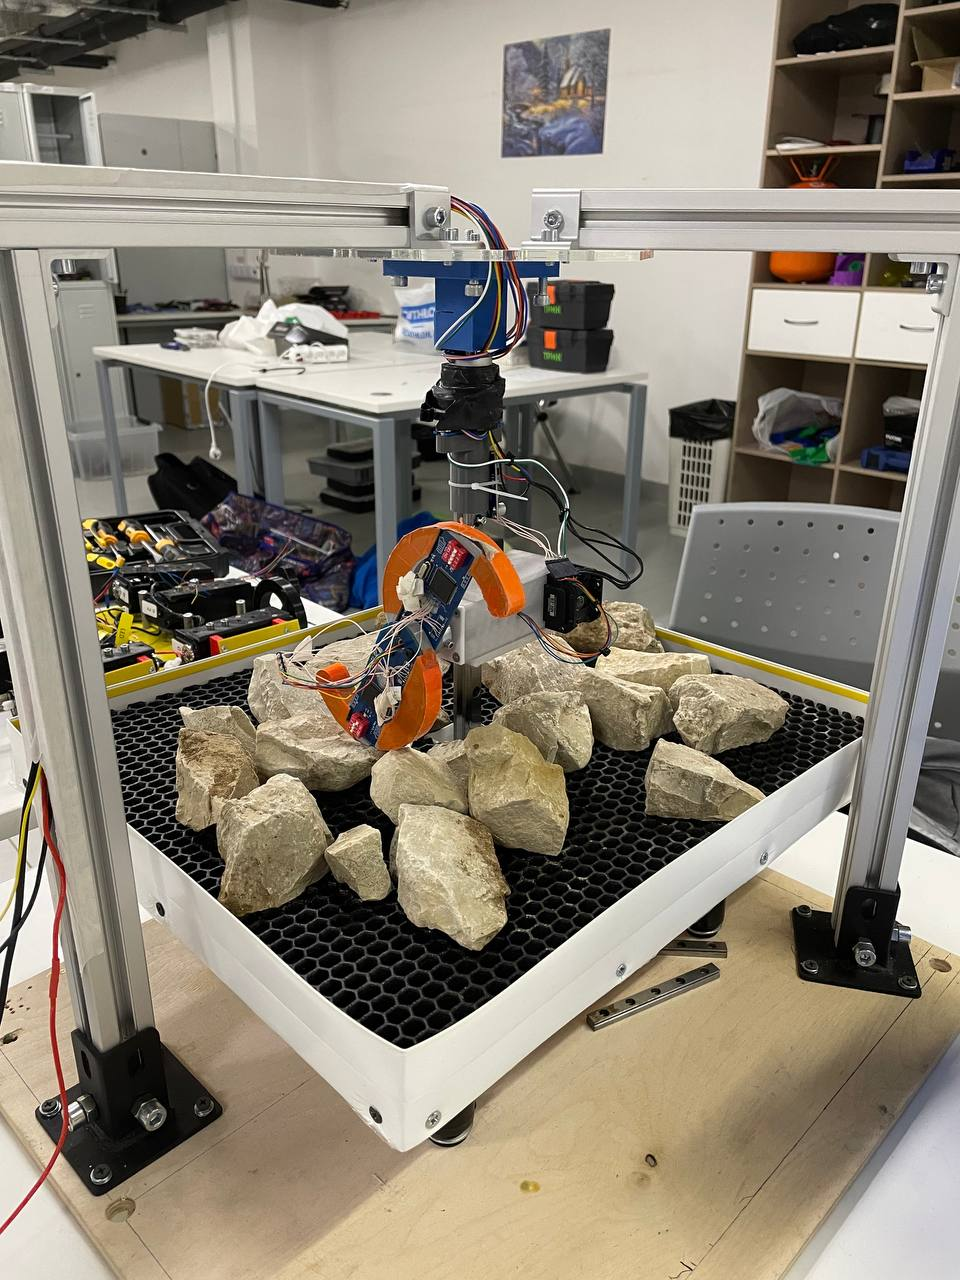
\includegraphics[height=6cm,width=1\textwidth,keepaspectratio]{s_shape_leg/view.jpg}}
            \caption*{Каменная гряда}
        \end{subfigure}
        \begin{subfigure}{0.5\textwidth}
            {\centering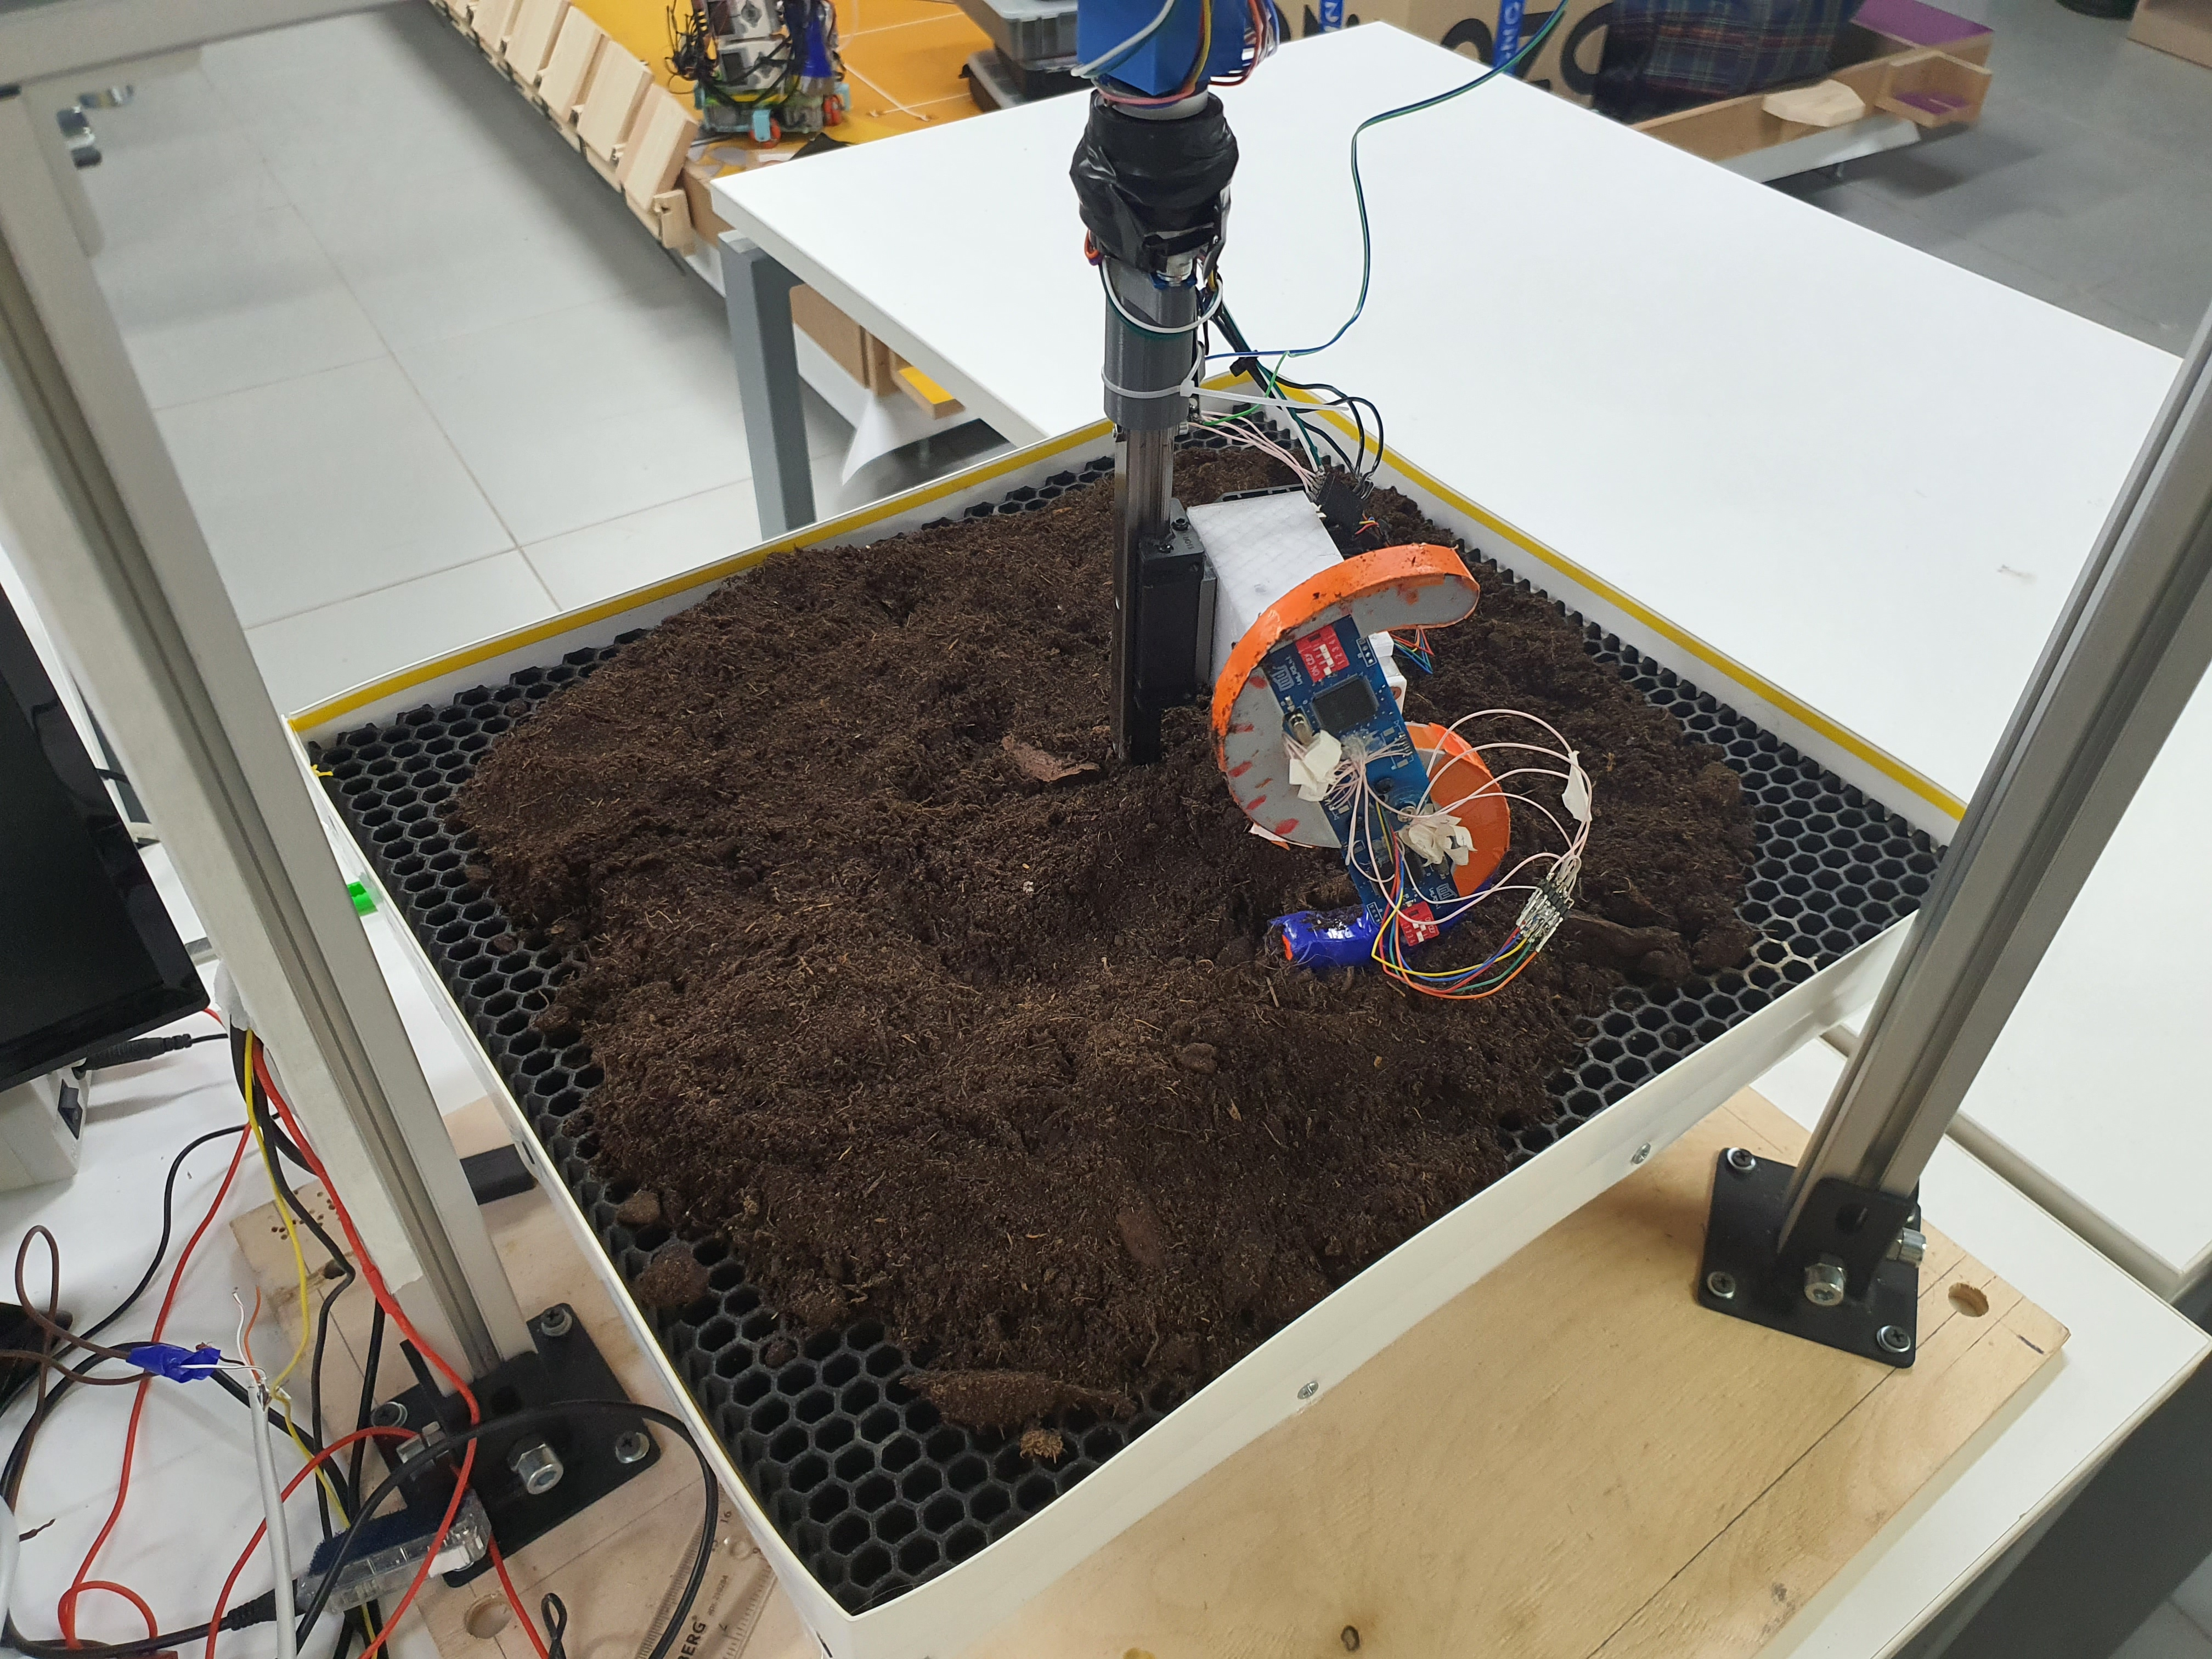
\includegraphics[height=6cm,width=1\textwidth,keepaspectratio]{s_shape_leg/mould.jpg}}
            \caption*{Земля}
        \end{subfigure}
    \end{figure}
\end{frame}


\begin{frame}[t]{Определение физических свойств поверхности}
    \framesubtitle{Данные с одного эксперимента}
    \begin{columns}[T,onlytextwidth]
        \begin{column}{0.60\textwidth}
            \begin{figure}[H]
                \centering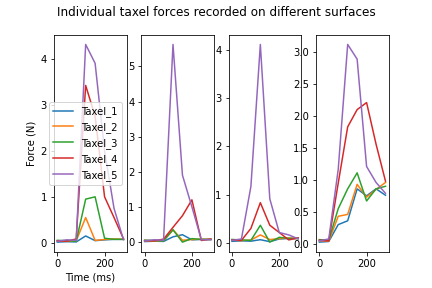
\includegraphics[height=5cm,width=1\textwidth,keepaspectratio]{s_shape_leg/TaxelIndForce.png}
            \end{figure}
        \end{column}
        \begin{column}{0.35\textwidth}
            \vspace{-1.4cm}
            \begin{figure}[H]
                    \centering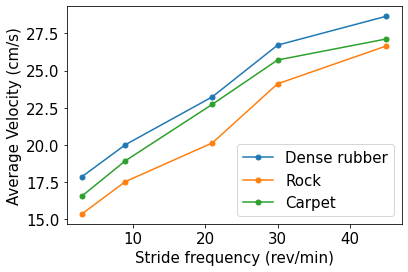
\includegraphics[height=3.8cm,width=1\textwidth,keepaspectratio]{s_shape_leg/avg_lin_vel_rev_min.png} 
            \end{figure}

            \resizebox{\linewidth}{!}{%
            \begin{tabular}{|c|c|c|c|c|} 
            \cline{3-5}
            \multicolumn{1}{l}{} & \multicolumn{1}{l|}{} & \multicolumn{3}{c|}{\textbf{Predicted Class}} \\ 
            \cline{3-5}
            \multicolumn{1}{l}{} &  & Rubber & Rock & Ground \\ 
            \hline
            \multirow{3}{*}{\rotcell{\textbf{True class}}} & Rubber & {\cellcolor[rgb]{0.741,0.843,0.929}}84.0\% & 2.56\% & 13.44\% \\ 
            \hhline{|~----|}
             & Rock & 20.1\% & {\cellcolor[rgb]{0.741,0.843,0.929}}67.8\% & 12.1\% \\ 
            \hhline{|~----|}
             & Ground & 1.0\% & 18.9\% & {\cellcolor[rgb]{0.741,0.843,0.929}}80.1\% \\
            \hline
            \end{tabular}
            }
            
        \end{column}
    \end{columns}
\end{frame}

% \begin{frame}[t]{Определение физических свойств поверхности}
%     \framesubtitle{Итог}
%     \large
%     \begin{itemize}
%         \item Возможность различать резиновую и каменистую поверхность.
%         \item Выбраны параметры классификации рельефа для машинного обучения:
%               \begin{itemize}
%                 \large
%                   \item Число оборотов в минуту
%                   \item Крутящий момент двигателя
%                   \item Ускорение от IMU
%                   \item Данные о силе, которые представлены как значение датчика\/сегмент, пиковая амплитуда, средняя амплитуда
%               \end{itemize}
%         \item Velostat датчик силы доказал свою работоспособность.
%     \end{itemize}
% \end{frame}

\begin{frame}[t]{Определение геометрических свойств поверхности}
    \framesubtitle{}
    {\large\begin{block}{Вопрос}
        Как создать плотное облако точек, используя разреженные данные об точках касания ног?
        \end{block}}
    {\large\begin{alertblock}{Ответ}
1. \textit{Создать полигональную сетку}, используя 2D триангуляцию Делоне (вогнутая оболочка) с использованием разреженных данных

2. \textit{Сгенерировать новые точки} из полигональной сетки

3. Вернуть плотное облако точек навигации навигации
        \end{alertblock}}
\end{frame}

\begin{frame}[t]{Определение геометрических свойств поверхности}
    \framesubtitle{Места проведения экспериментов}
    \vspace{-15pt}
    \begin{figure}[H]
        \begin{subfigure}[t]{0.49\textwidth}
            \centering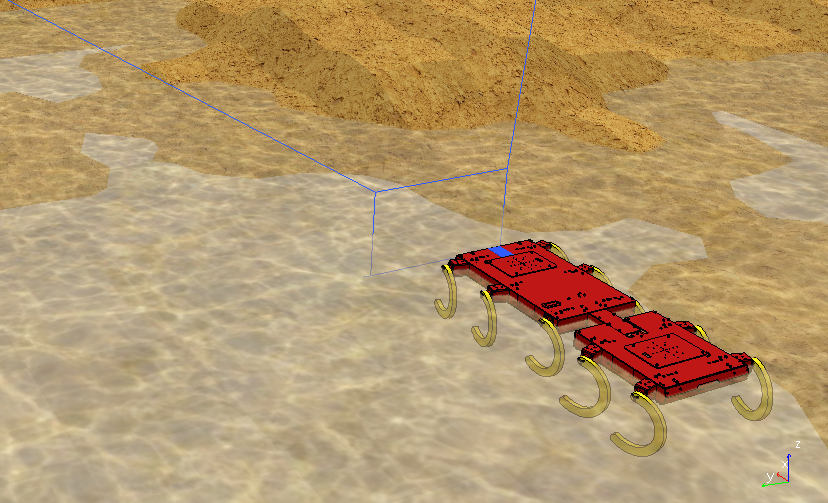
\includegraphics[height=5cm,width=1\textwidth,keepaspectratio]{coppelia_sim.png}
            \caption*{CoppeliaSim симулятор,\\ \textbf{4th gen} СтриРус}
        \end{subfigure}
        \begin{subfigure}[t]{0.49\textwidth}
            \centering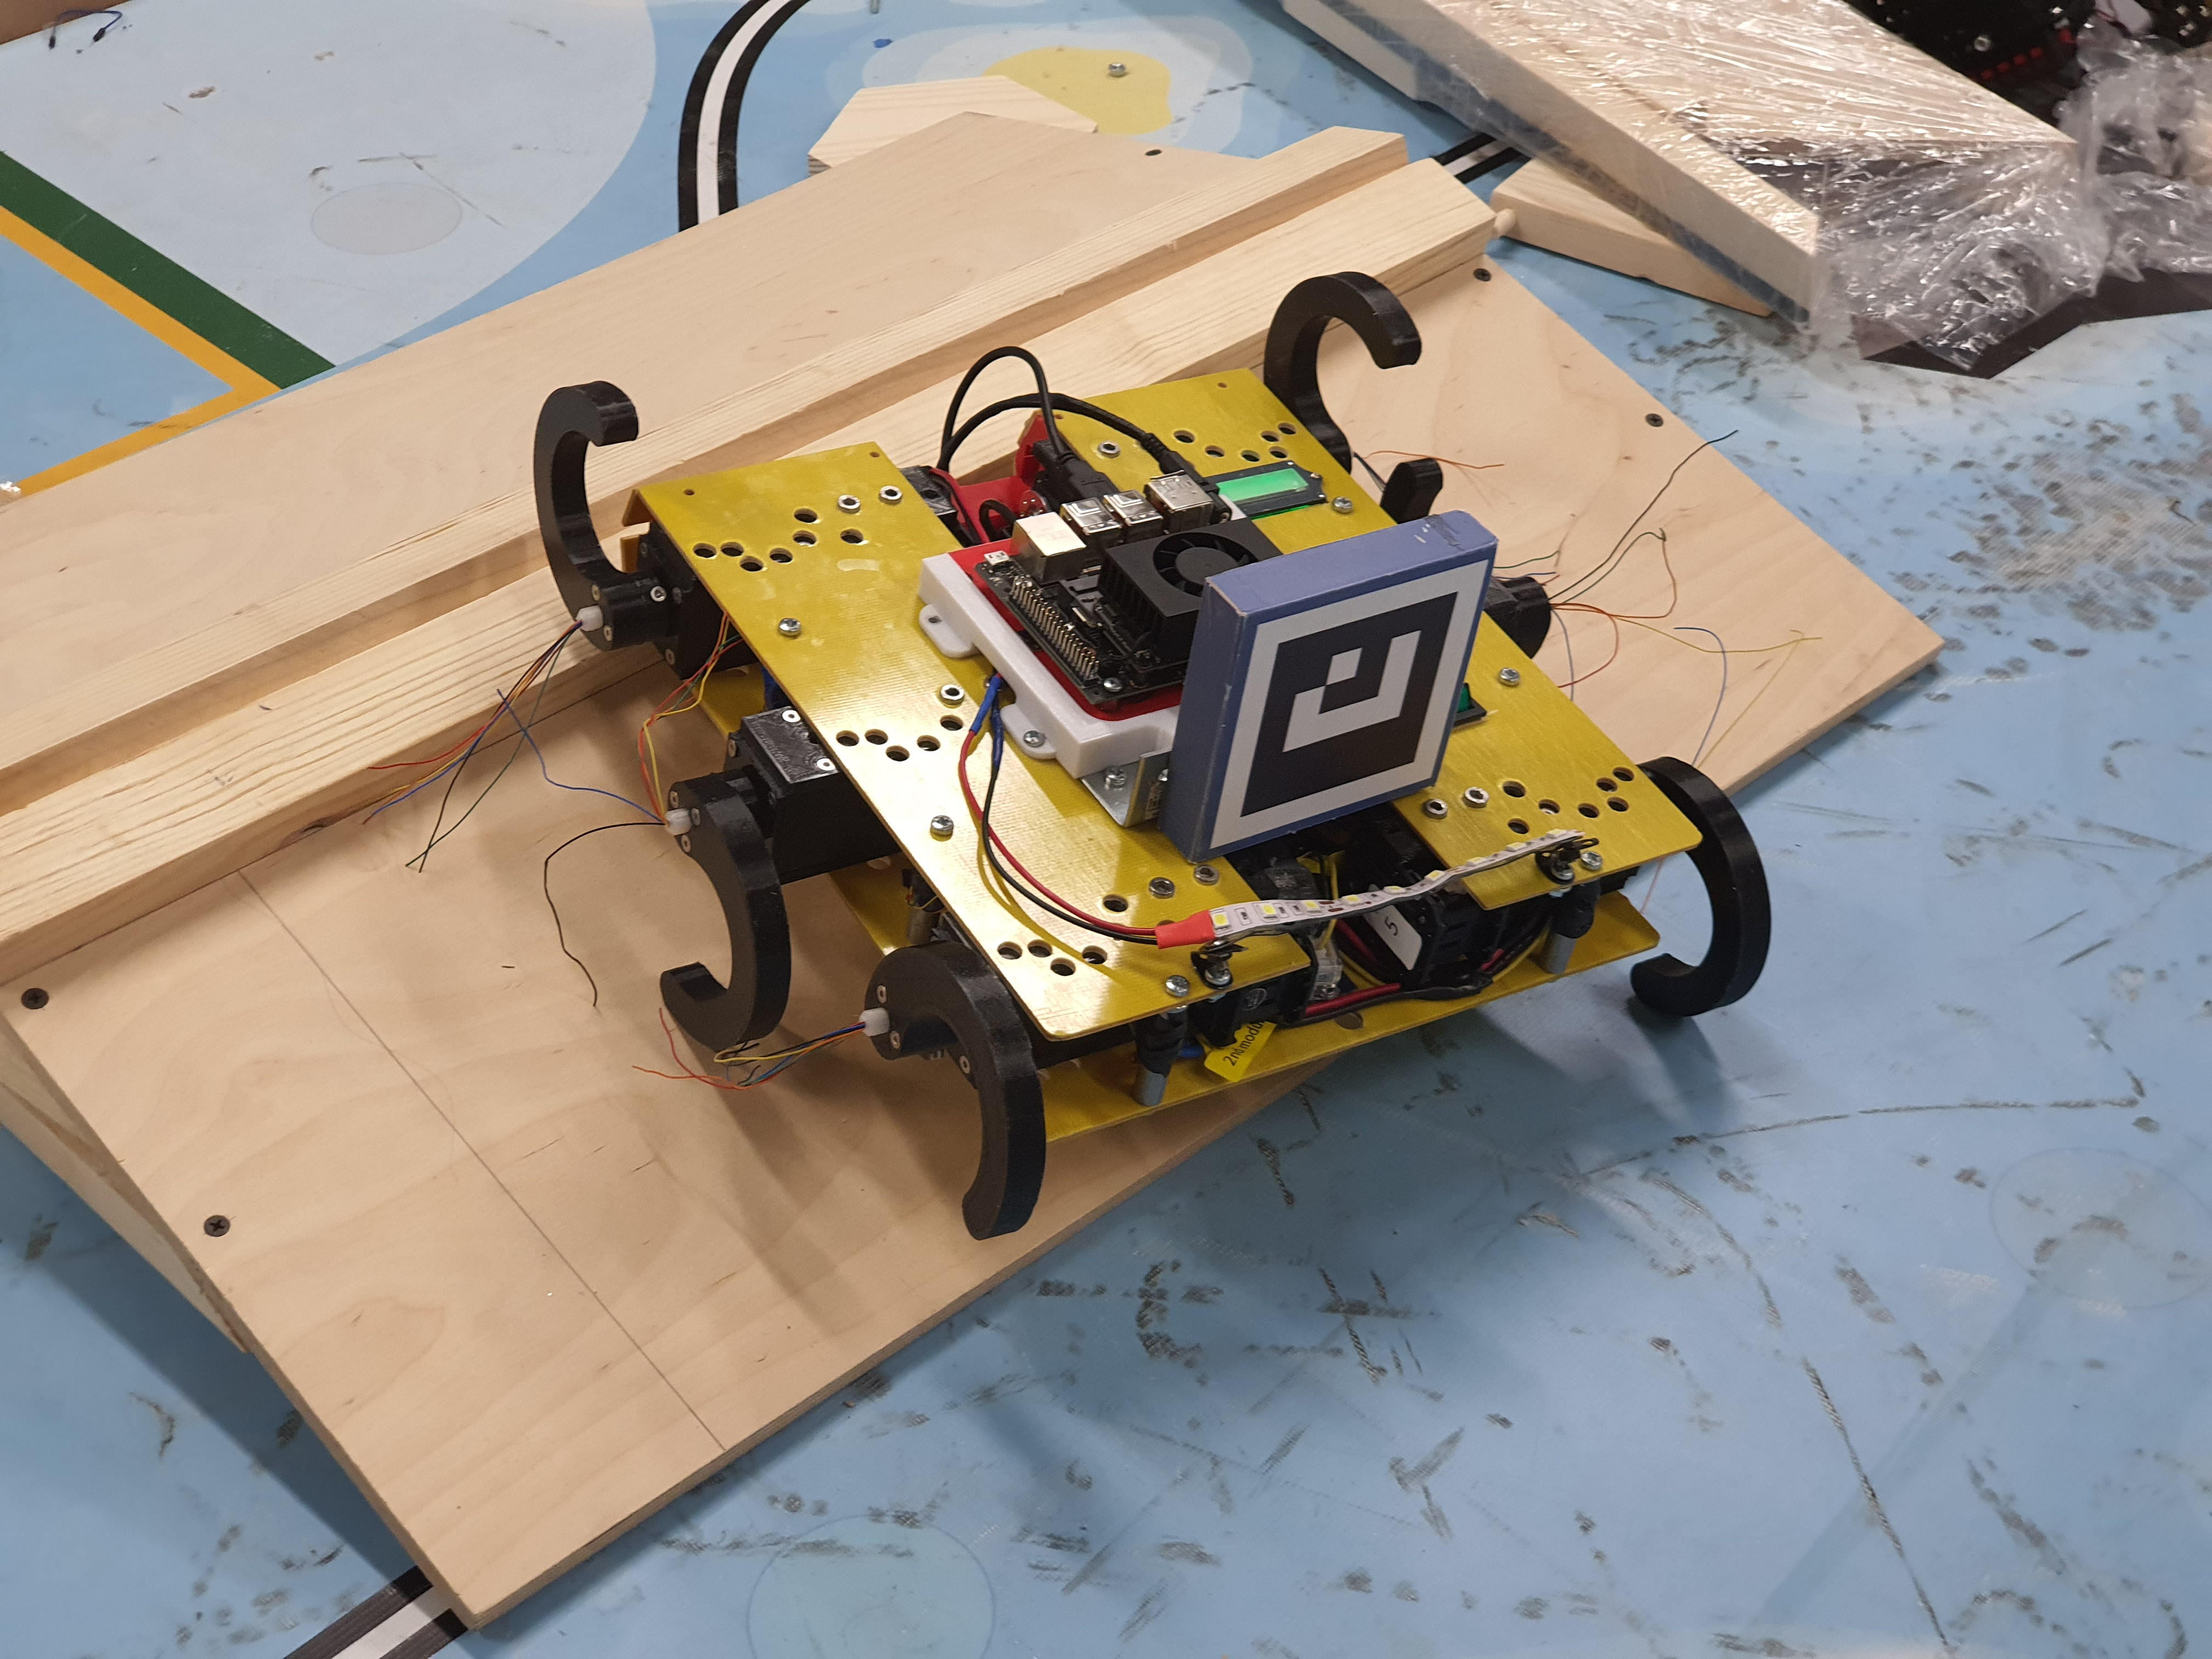
\includegraphics[height=5cm,width=1\textwidth,keepaspectratio]{rl_sim.JPG}
            \caption*{Натурные испытания,\\ \textbf{3th+ gen} СтриРус}
        \end{subfigure}
    \end{figure}
\end{frame}

\begin{frame}[t]{Определение геометрических свойств поверхности}
    \framesubtitle{Триангуляция Делоне}
    \vspace{-0.2cm}
    \begin{figure}[H]
        \centering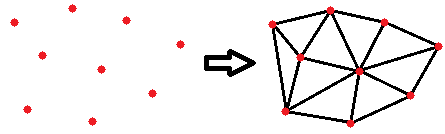
\includegraphics[height=6cm,width=1\textwidth,keepaspectratio]{delone_idea.png}
        \caption*{2D триангуляция Делоне (Выпуклая оболочка) \\ \textbf{От облака точек к полигональной сетке}}
        \label{fig:delone_idea.png}
    \end{figure}
\end{frame}

\begin{frame}[t]{Определение геометрических свойств поверхности}
    \framesubtitle{Почему важно использовать вогнутую оболочку (модификация Делоне)}
    \vspace{-15pt}
    \begin{figure}[H]
        \begin{subfigure}[t]{0.3\textwidth}
            \centering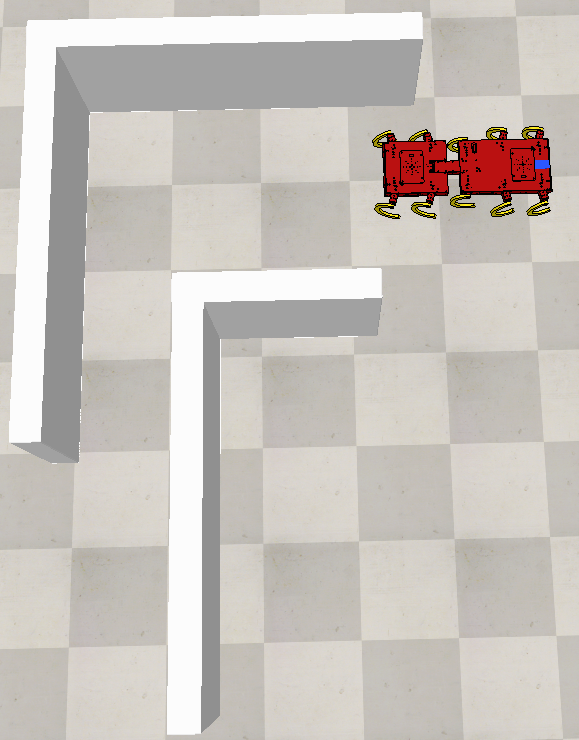
\includegraphics[height=5cm,width=1\textwidth,keepaspectratio]{convex_terr.png}
            \caption*{Пример поверхности}
            \label{fig:convex_terr.png}
        \end{subfigure}
        \hfill
        \begin{subfigure}[t]{0.33\textwidth}
                \centering
                 \begin{tikzpicture}
                    % Include the image in a node
                    \node [above right, inner sep=0] (image) at (0,0) 
                    {\centering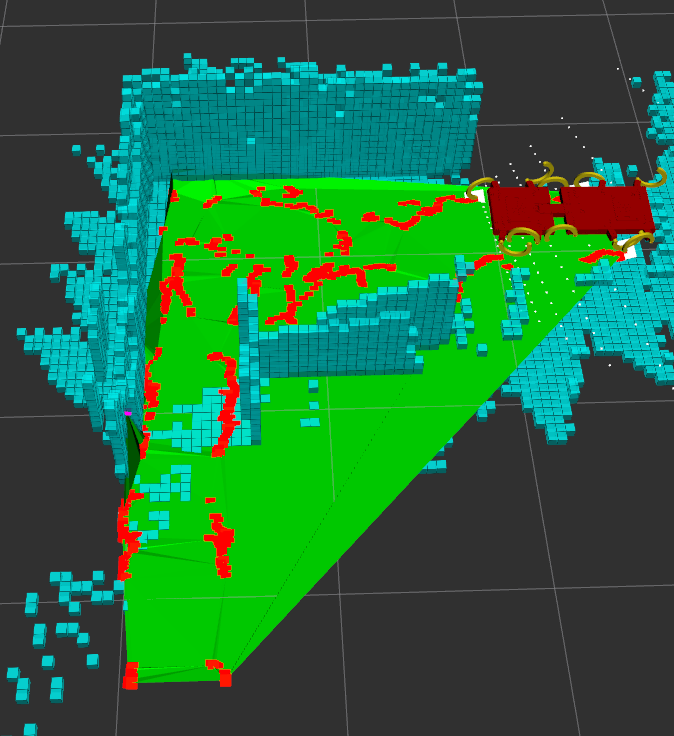
\includegraphics[height=6cm,width=1\textwidth,keepaspectratio]{conv_convex.png}};          
                    % Create scope with normalized axes
                    \begin{scope}[
                        x={($ 0.1*(image.south east)$)},
                        y={($ 0.1*(image.north west)$)}]
                        % Grid and axes' labels
                        % \draw[lightgray,step=1] (image.south west) grid (image.north east);
                        % \foreach \x in {0,1,...,10} { \node [below] at (\x,0) {\x}; }
                        % \foreach \y in {0,1,...,10} { \node [left] at (0,\y) {\y};}
             
                        % Labels
                        \draw[stealth-, very thick,green] (5.2,3.5) -- ++(1,-1)
                        node[rounded corners=3pt,right,black,fill=white]{\tiny Generated mesh};
                        
                        \draw[stealth-, very thick,green] (5.5,5.5) -- (7.4,4)
                        node[rounded corners=3pt,right,black,fill=white]{\tiny Lidar data};
                        
                        
                        \draw[stealth-, very thick,green] (3.4,0.8) -- (5,1);            
                        \draw[stealth-, very thick,green] (3.4,2.6) -- (5,1)
                        node[rounded corners=3pt,right,black,fill=white]{\tiny Cloud of contact points};
                    \end{scope}
                \end{tikzpicture}
                \caption*{Выпуклая оболочка}
                \label{fig:conv_convex.png}
        \end{subfigure}
        \hfill
        \begin{subfigure}[t]{0.33\textwidth}
            \centering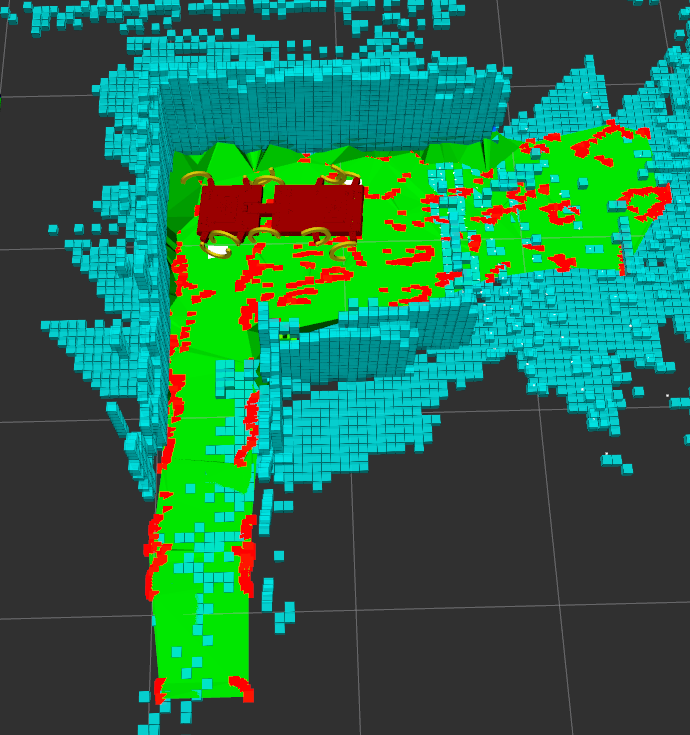
\includegraphics[height=6cm,width=1\textwidth,keepaspectratio]{conv_concave.png}
            \caption*{Вогнутая оболочка}
            \label{fig:conv_concave.png}
        \end{subfigure}

    \end{figure}
\end{frame}

\begin{frame}[t]{Определение геометрических свойств поверхности}
    \framesubtitle{Результат: Маршрут, полигональная сетка}
    \vspace{-15pt}
            \begin{figure}[H]
                \begin{subfigure}[t]{0.36\textwidth}
                    \centering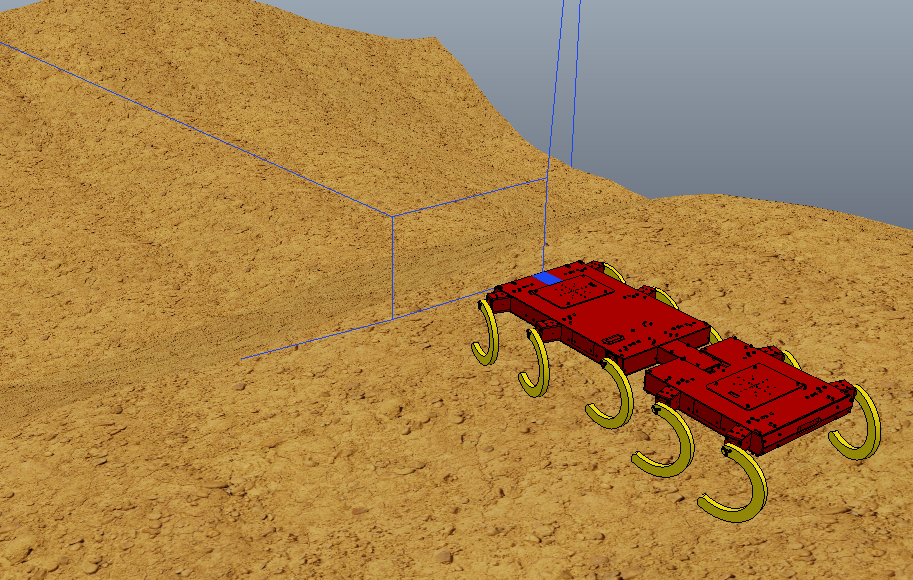
\includegraphics[height=5cm,width=1\textwidth,keepaspectratio]{terrain_wo_water.png}
                    \caption*{Начало маршрута}
                \end{subfigure}
                \begin{subfigure}[t]{0.36\textwidth}
                    \centering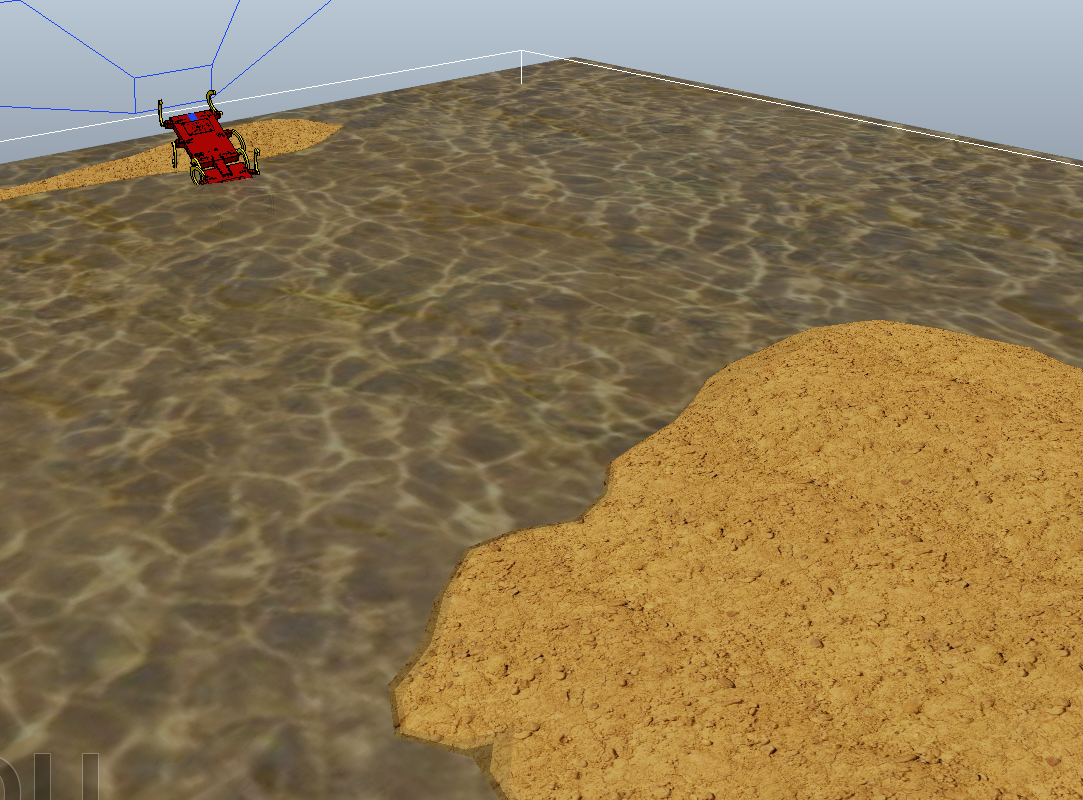
\includegraphics[height=5cm,width=1\textwidth,keepaspectratio]{terrain_w_water_end.png}
                    \caption*{Конец маршрута}
                \end{subfigure}
                \begin{subfigure}[t]{0.26\textwidth}
                    \centering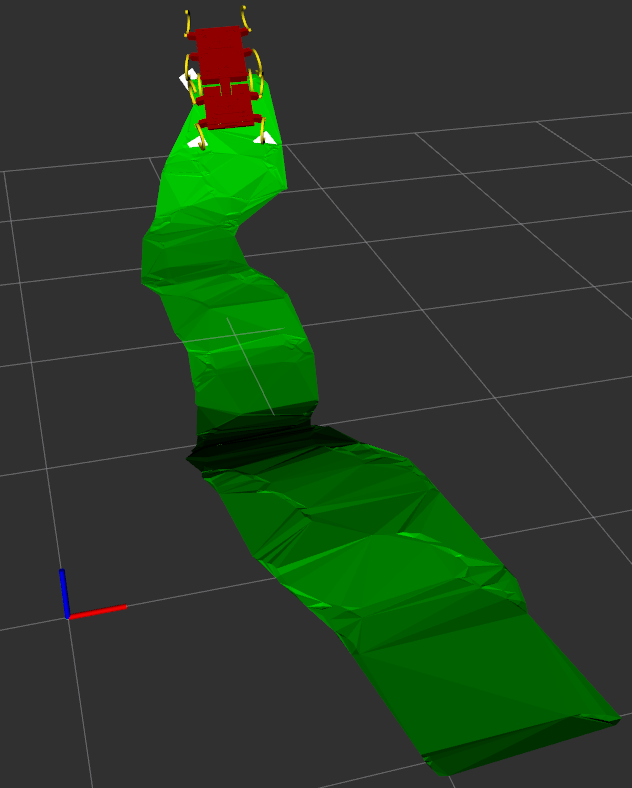
\includegraphics[height=5cm,width=1\textwidth,keepaspectratio]{mesh_rviz.png}
                    \caption*{Созданная сетка}
                \end{subfigure}
            \end{figure}  


\end{frame}

\begin{frame}[t]{Определение геометрических свойств поверхности}
    \framesubtitle{Метрики Cloud2Cloud и Cloud2Mesh}
    \vspace{-15pt}
    \begin{figure}[H]
        \begin{subfigure}[t]{0.49\textwidth}
            \centering
             \begin{tikzpicture}
                % Include the image in a node
                \node [above right, inner sep=0] (image) at (0,0) 
                {\centering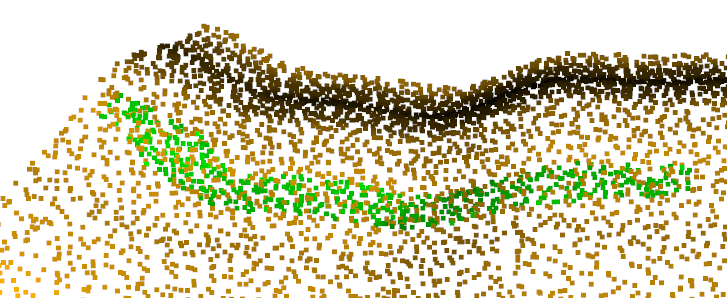
\includegraphics[height=2.8cm,width=1\textwidth,keepaspectratio]{sampled_pcd.png}};          
                % Create scope with normalized axes
                \begin{scope}[
                    x={($ 0.1*(image.south east)$)},
                    y={($ 0.1*(image.north west)$)}]
                    % Grid and axes' labels
                    % \draw[lightgray,step=1] (image.south west) grid (image.north east);
                    % \foreach \x in {0,1,...,10} { \node [below] at (\x,0) {\x}; }
                    % \foreach \y in {0,1,...,10} { \node [left] at (0,\y) {\y};}
         
                    % Labels
                    \draw[stealth-, very thick,green] (3,8) -- (2,8.5);
                    \draw[stealth-, very thick,green] (1,5.5) -- (2,8.5)
                    node[rounded corners=3pt,above,black,fill=white]{\tiny Ground Truth Point Cloud};
         
                    \draw[stealth-, very thick,green] (5.5,3) -- (5.5,8.5)
                    node[rounded corners=3pt,above,black,fill=white]{\tiny Generated Point Cloud};
                \end{scope}
            \end{tikzpicture}
            % \caption*{Наложенные облака точек}
            \label{fig:sampled_pcd.png}
    \end{subfigure}
    \begin{subfigure}[t]{0.49\textwidth}
        \centering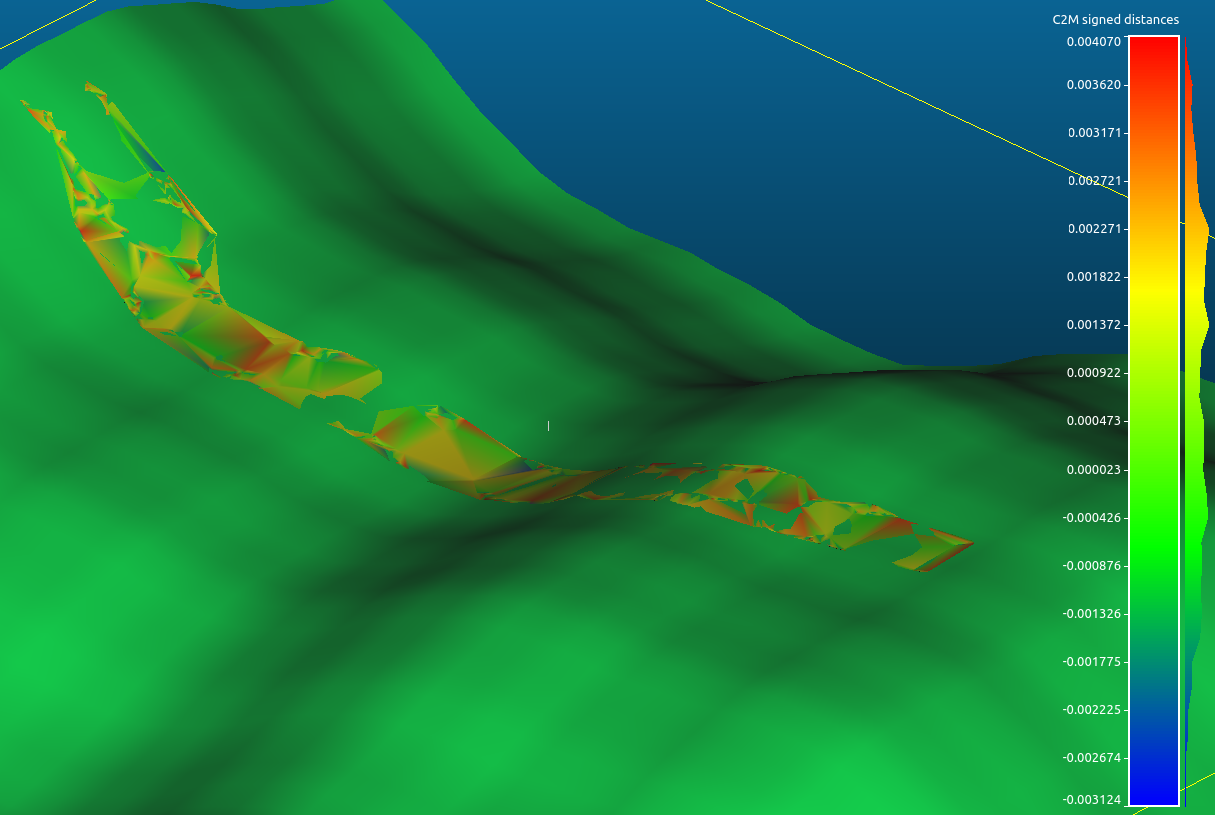
\includegraphics[height=2.8cm,width=1\textwidth,keepaspectratio]{mesh_comp.png}
        % \caption*{Наложенные сетки}
    \end{subfigure}

        \begin{subfigure}[t]{0.49\textwidth}
            \centering\includegraphics[height=2.6cm,width=1\textwidth,keepaspectratio]{pcd_hist.png}
            \caption*{Гистограмма ошибок C2C}
        \end{subfigure}
        \begin{subfigure}[t]{0.49\textwidth}
            \centering\includegraphics[height=2.6cm,width=1\textwidth,keepaspectratio]{mesh_hist.png}
            \caption*{Гистограмма ошибок C2M}
        \end{subfigure}
    \end{figure}
\end{frame}

\begin{frame}[t]{Определение геометрических свойств поверхности}
    \framesubtitle{Результат: Натурные испытания, Видео}
    \vspace{-0.5cm}
    \begin{figure}[H]
        \begin{subfigure}[t]{0.49\textwidth}
            % \href{run:./videos/big_angle2.mp4}{
            \href{https://youtu.be/2dxHHTG4psQ}{
                \centering\includegraphics[height=6cm,width=1\textwidth,keepaspectratio]{real_robot_mesh_video_preview.png}}
            \caption*{Робот проходит препятствие}
        \end{subfigure}
        \begin{subfigure}[t]{0.49\textwidth}
            \centering\includegraphics[height=6cm,width=1\textwidth,keepaspectratio]{real_mesh.jpg}
            \caption*{Полигональная сетка, полученная с помощью ног}
        \end{subfigure}
    \end{figure}
\end{frame}

% \begin{frame}[t]{Определение геометрических свойств поверхности}
%     \framesubtitle{Итог}
%     \large
%     \begin{itemize}
%         \item Карта может быть построена с помощью \textit{вогнутой оболочки 2D триангуляции Делоне}, где входными данными являются \textit{точки касания, определенные датчиком силы}.
%         \item \textit{Симулятор} (Среднее значение среднеквадратичной ошибки): \begin{itemize}
%             \large
%                   \item При сравнении облаков точек составляет около 5 см.
%                   \item При сравнении сеткок составляет около 1 см.
%               \end{itemize}
%         \item \textit{Натурный эксперимент} (---//---): \begin{itemize}
%             \large
%                   \item При сравнении облаков точек составляет около 8 см.
%                         % \item Среднее значение. RMSE при сравнении сетки составляет около 1 см.
%               \end{itemize}
%               \textit{Это приемлимая точность для такой задачи.}
%     \end{itemize}
% \end{frame}


\begin{frame}[t]{Глобальный итог}
    \framesubtitle{}
    \large
    \vspace{-0.5cm}
    \begin{figure}[H]
        \begin{subfigure}[t]{0.49\textwidth}
            \centering\includegraphics[height=2.5cm,width=1\textwidth,keepaspectratio]{strirus_3.JPG}
            \caption*{1. Структурный синтез}
        \end{subfigure}
        \begin{subfigure}[t]{0.49\textwidth}
            \centering\includegraphics[height=2.5cm,width=1\textwidth,keepaspectratio]{velostat_sensor_look.JPG}
            \caption*{2. Датчик силы на основе Velostat}
        \end{subfigure}
    
        \begin{subfigure}[t]{0.49\textwidth}
            \centering\includegraphics[height=2.5cm,width=1\textwidth,keepaspectratio]{s_shape_leg/s_leg_setup.JPG}
            \caption*{3. Определение поверхности}
        \end{subfigure}
        \begin{subfigure}[t]{0.49\textwidth}
            \centering\includegraphics[height=2.5cm,width=1\textwidth,keepaspectratio]{conv_concave.png}
            \caption*{4. Ножное картографирование}
        \end{subfigure}
    \end{figure}
\end{frame}

\begin{frame}[t]{Результаты решения задач}
    \framesubtitle{}
    \vspace{-0.7cm}
        \begin{columns}[T,onlytextwidth]
            \begin{column}{0.48\textwidth}
                \begin{block}{Научных задач (научная новизна)}
                    1. Методика \textbf{подбора количества ног для шагающих цикловых движителей}.
                    
                    2. Методика \textbf{характеризации датчика}, когда площадь касания нагрузки меньше, чем размеры датчика.
                    
                    3. Методика \textbf{калибровки} и \textbf{алгоритм определения типа поверхности}.
                    
                    4. Методика определения \textbf{геометрических свойств местности}.   
                        
                    \end{block}
            \end{column}
            \begin{column}{0.48\textwidth}
                \begin{alertblock}{Инженерных задач}
     1. \textbf{Шагающий цикловой движитель} с одной степенью свободы в ноге.
    
    2. \textbf{Выбраны, откалиброваны и установлены не оптические сенсоры} для определения свойств поверхности.
    
    3. Алгоритм \textbf{определения типа поверхности}.
    
    4. Алгоритм \textbf{картографирования местности} с помощью \textbf{пальпирования} ногами робота.
    
                \end{alertblock}
            \end{column}
        \end{columns}
    \end{frame}

\begin{frame}[t]{Результаты интеллектуальной деятельности}
\framesubtitle{}
\large
\begin{itemize}
    \item \textit{Количество публикаций} 
    \begin{itemize}
        \large
        \item \textbf{1.5} --- журналы, рекомендованных ВАК
        \item \textbf{3} --- журналы, индексируемые в Scopus (2 работы Q2)
        \item \textbf{9} --- РИНЦ
        \item \textbf{2} --- готовятся к публикации в Scopus
    \end{itemize}
    \item \textbf{8} --- Зарегистрированных программ для ЭВМ
    \item \textbf{3} --- Выигранных гранта (Умник, ЦНТИ, РФФИ)
\end{itemize}
\end{frame}


% \fbckg{fibeamer/figs/last_page.png}
% \frame[plain]{}
% \fbckg{fibeamer/figs/common.png}

\end{document}